\documentclass[12pt]{article}
\usepackage[margin=1in]{geometry}
\usepackage{amsmath}
\usepackage{amsfonts}
\usepackage{amssymb}
\usepackage{tikz-cd}
\usepackage{quiver}
\usepackage{enumitem}
\usepackage{float}
\usepackage{hyperref}

\title{Data Science 1 - HW 3}
\author{CSYS 5870, Fall 2025}
\date{September 26, 2025}

\begin{document}

\maketitle

\section*{Question 1: Revisiting a Previous Visualization}
\subsection*{Part 1: Constructing a hand drawn image}

\begin{figure}[htbp]
    \centering
    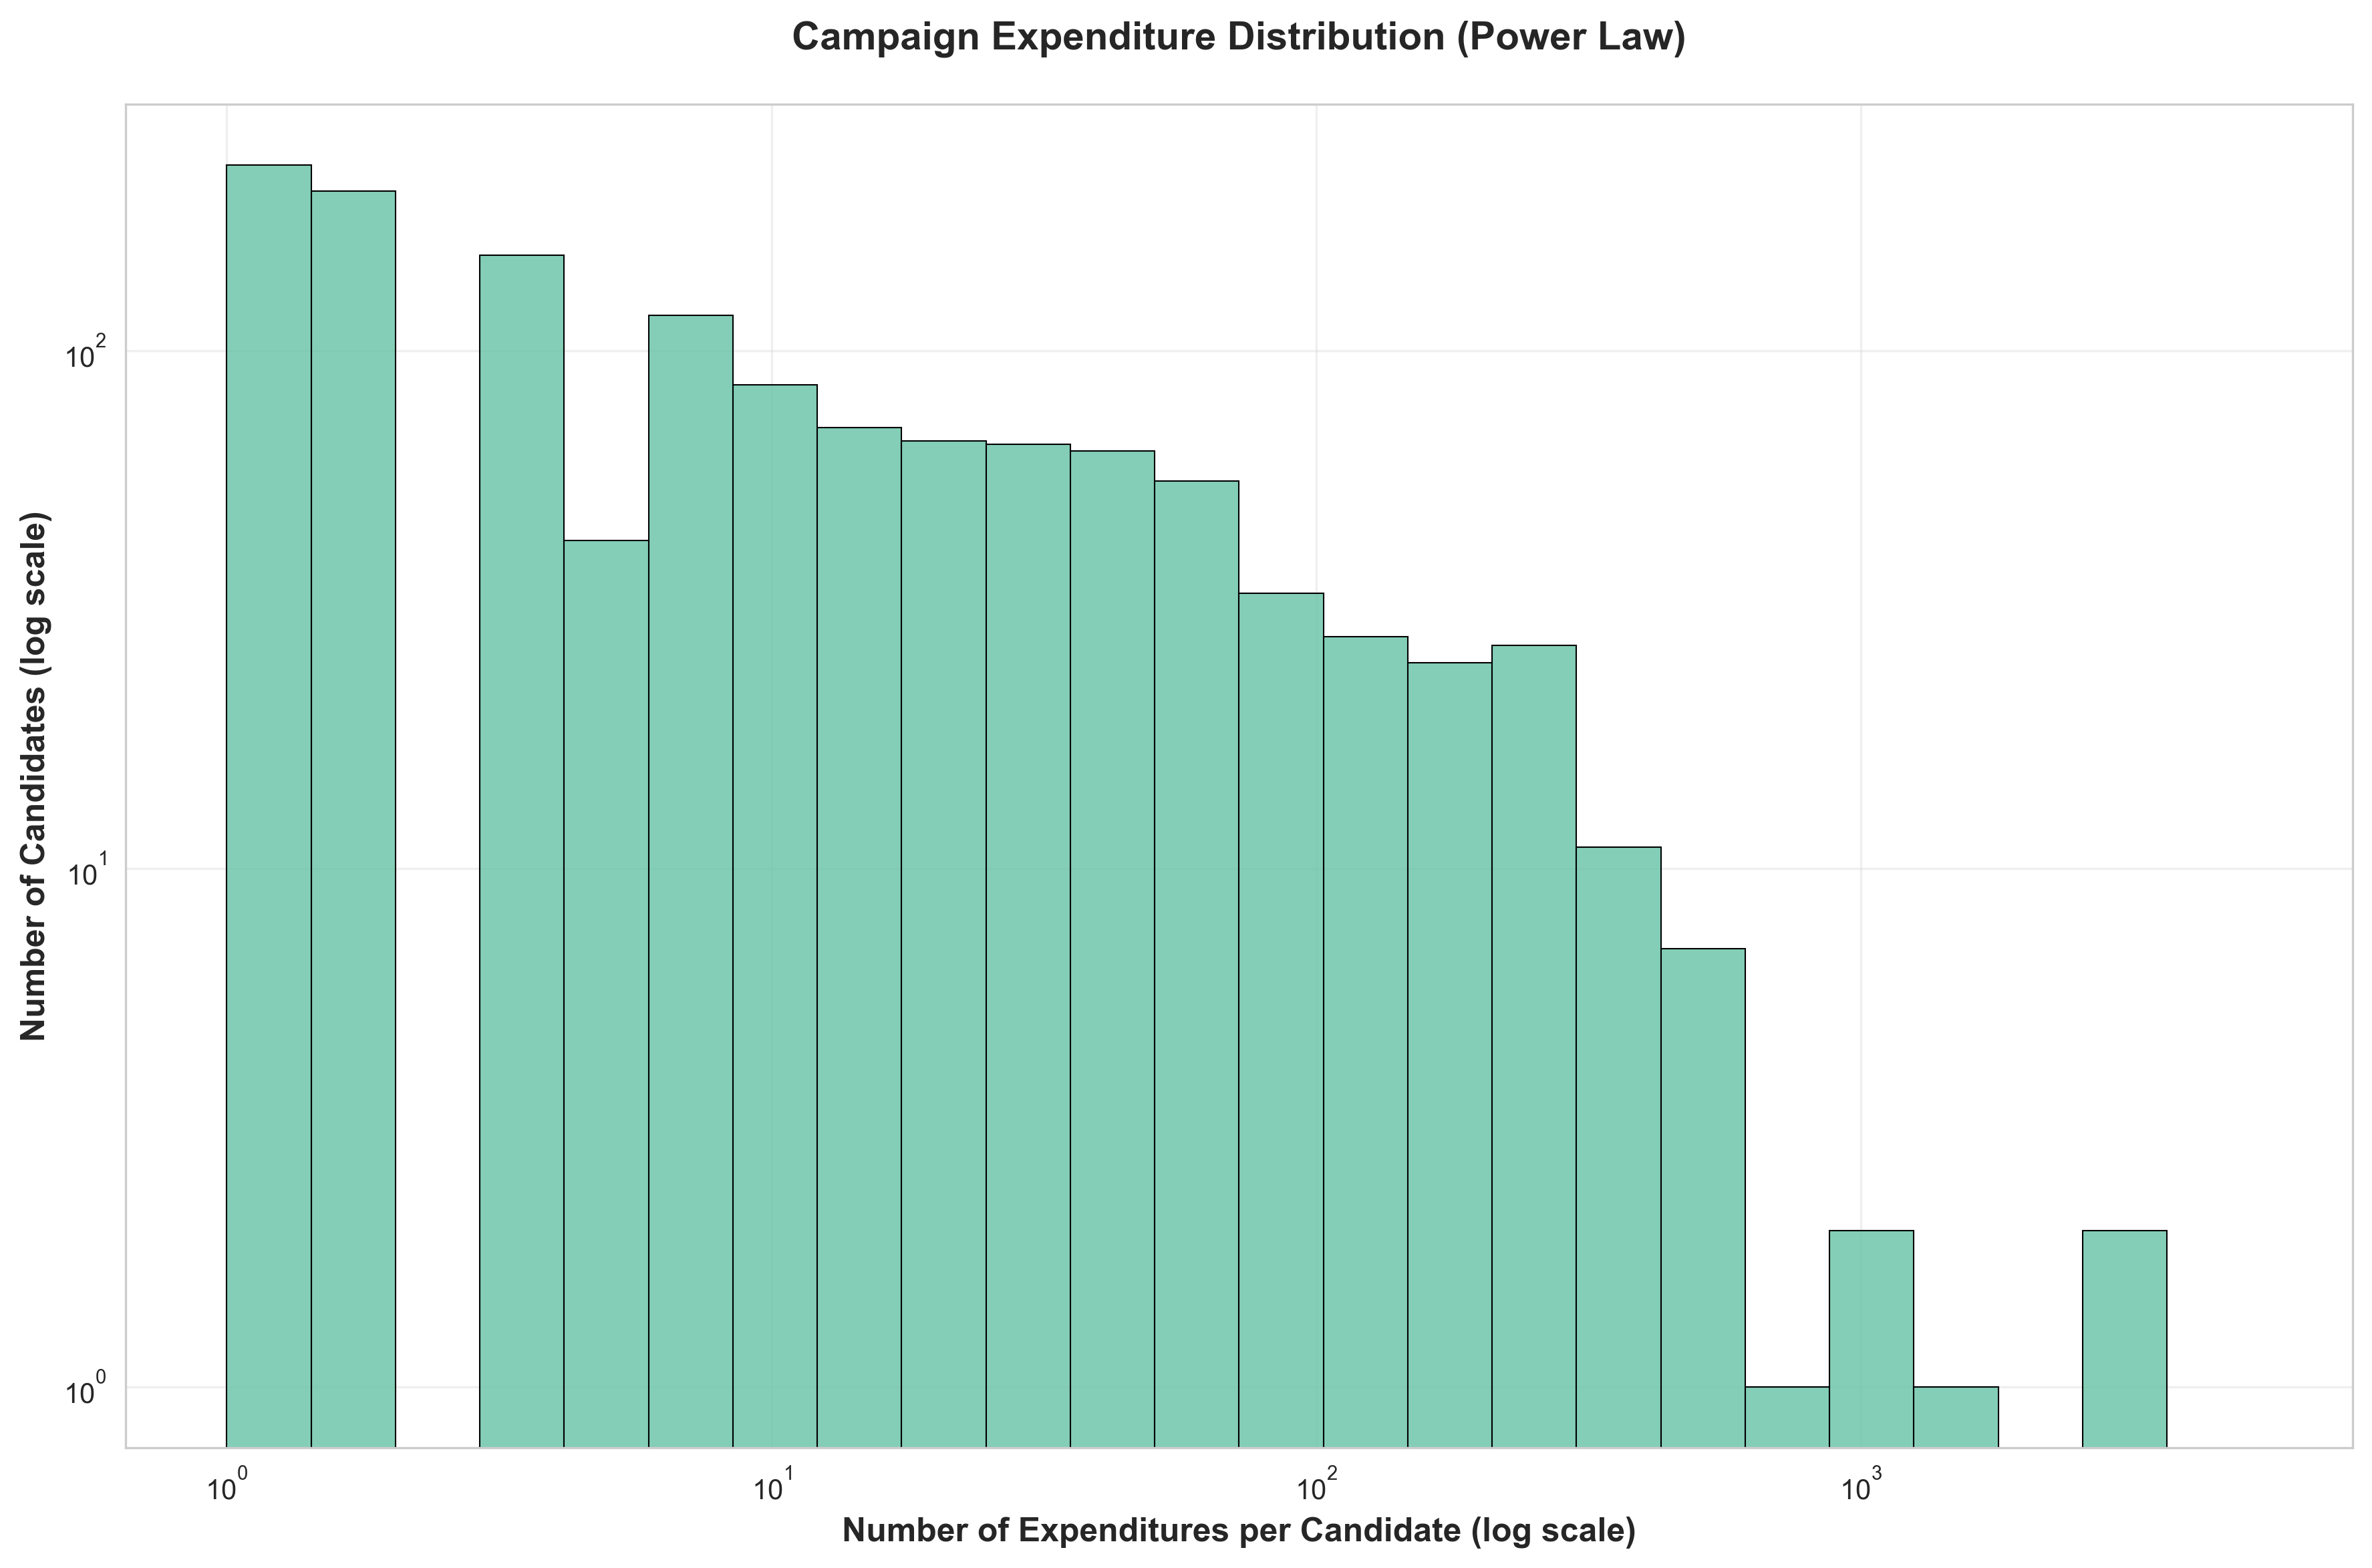
\includegraphics[width=0.8\linewidth]{power_law.png}
    \caption{Image selected to revisit}
    \label{fig:myfigure}
\end{figure}

This plot was an attempt at conveying the idea that campaign expenditures are dominated by 2 individuals. The feedback I received is that the image is confusing. "Perhaps you should flip the axis." The idea was that the tail would be more defined. The bigger question was around the "so what?". 

\begin{itemize}
    \item Why is this distribution important?
    \item What is an expenditure?
    \item How do these expenditures breakdown across candidate/election type?
    \item How do expenditures translate to dollars spent?
    \item How can we visualize how dollars are spent on different types of expenditures?
\end{itemize}

In trying to answer these questions with a hand drawn picture, I tried to focus on how a visualization might flow from panel to panel. My inspiration came from Claus Wilke's "compound figures" - specifically I tried to "employ a consistent visual language" in telling my story.

\begin{figure}[htbp]
    \centering
    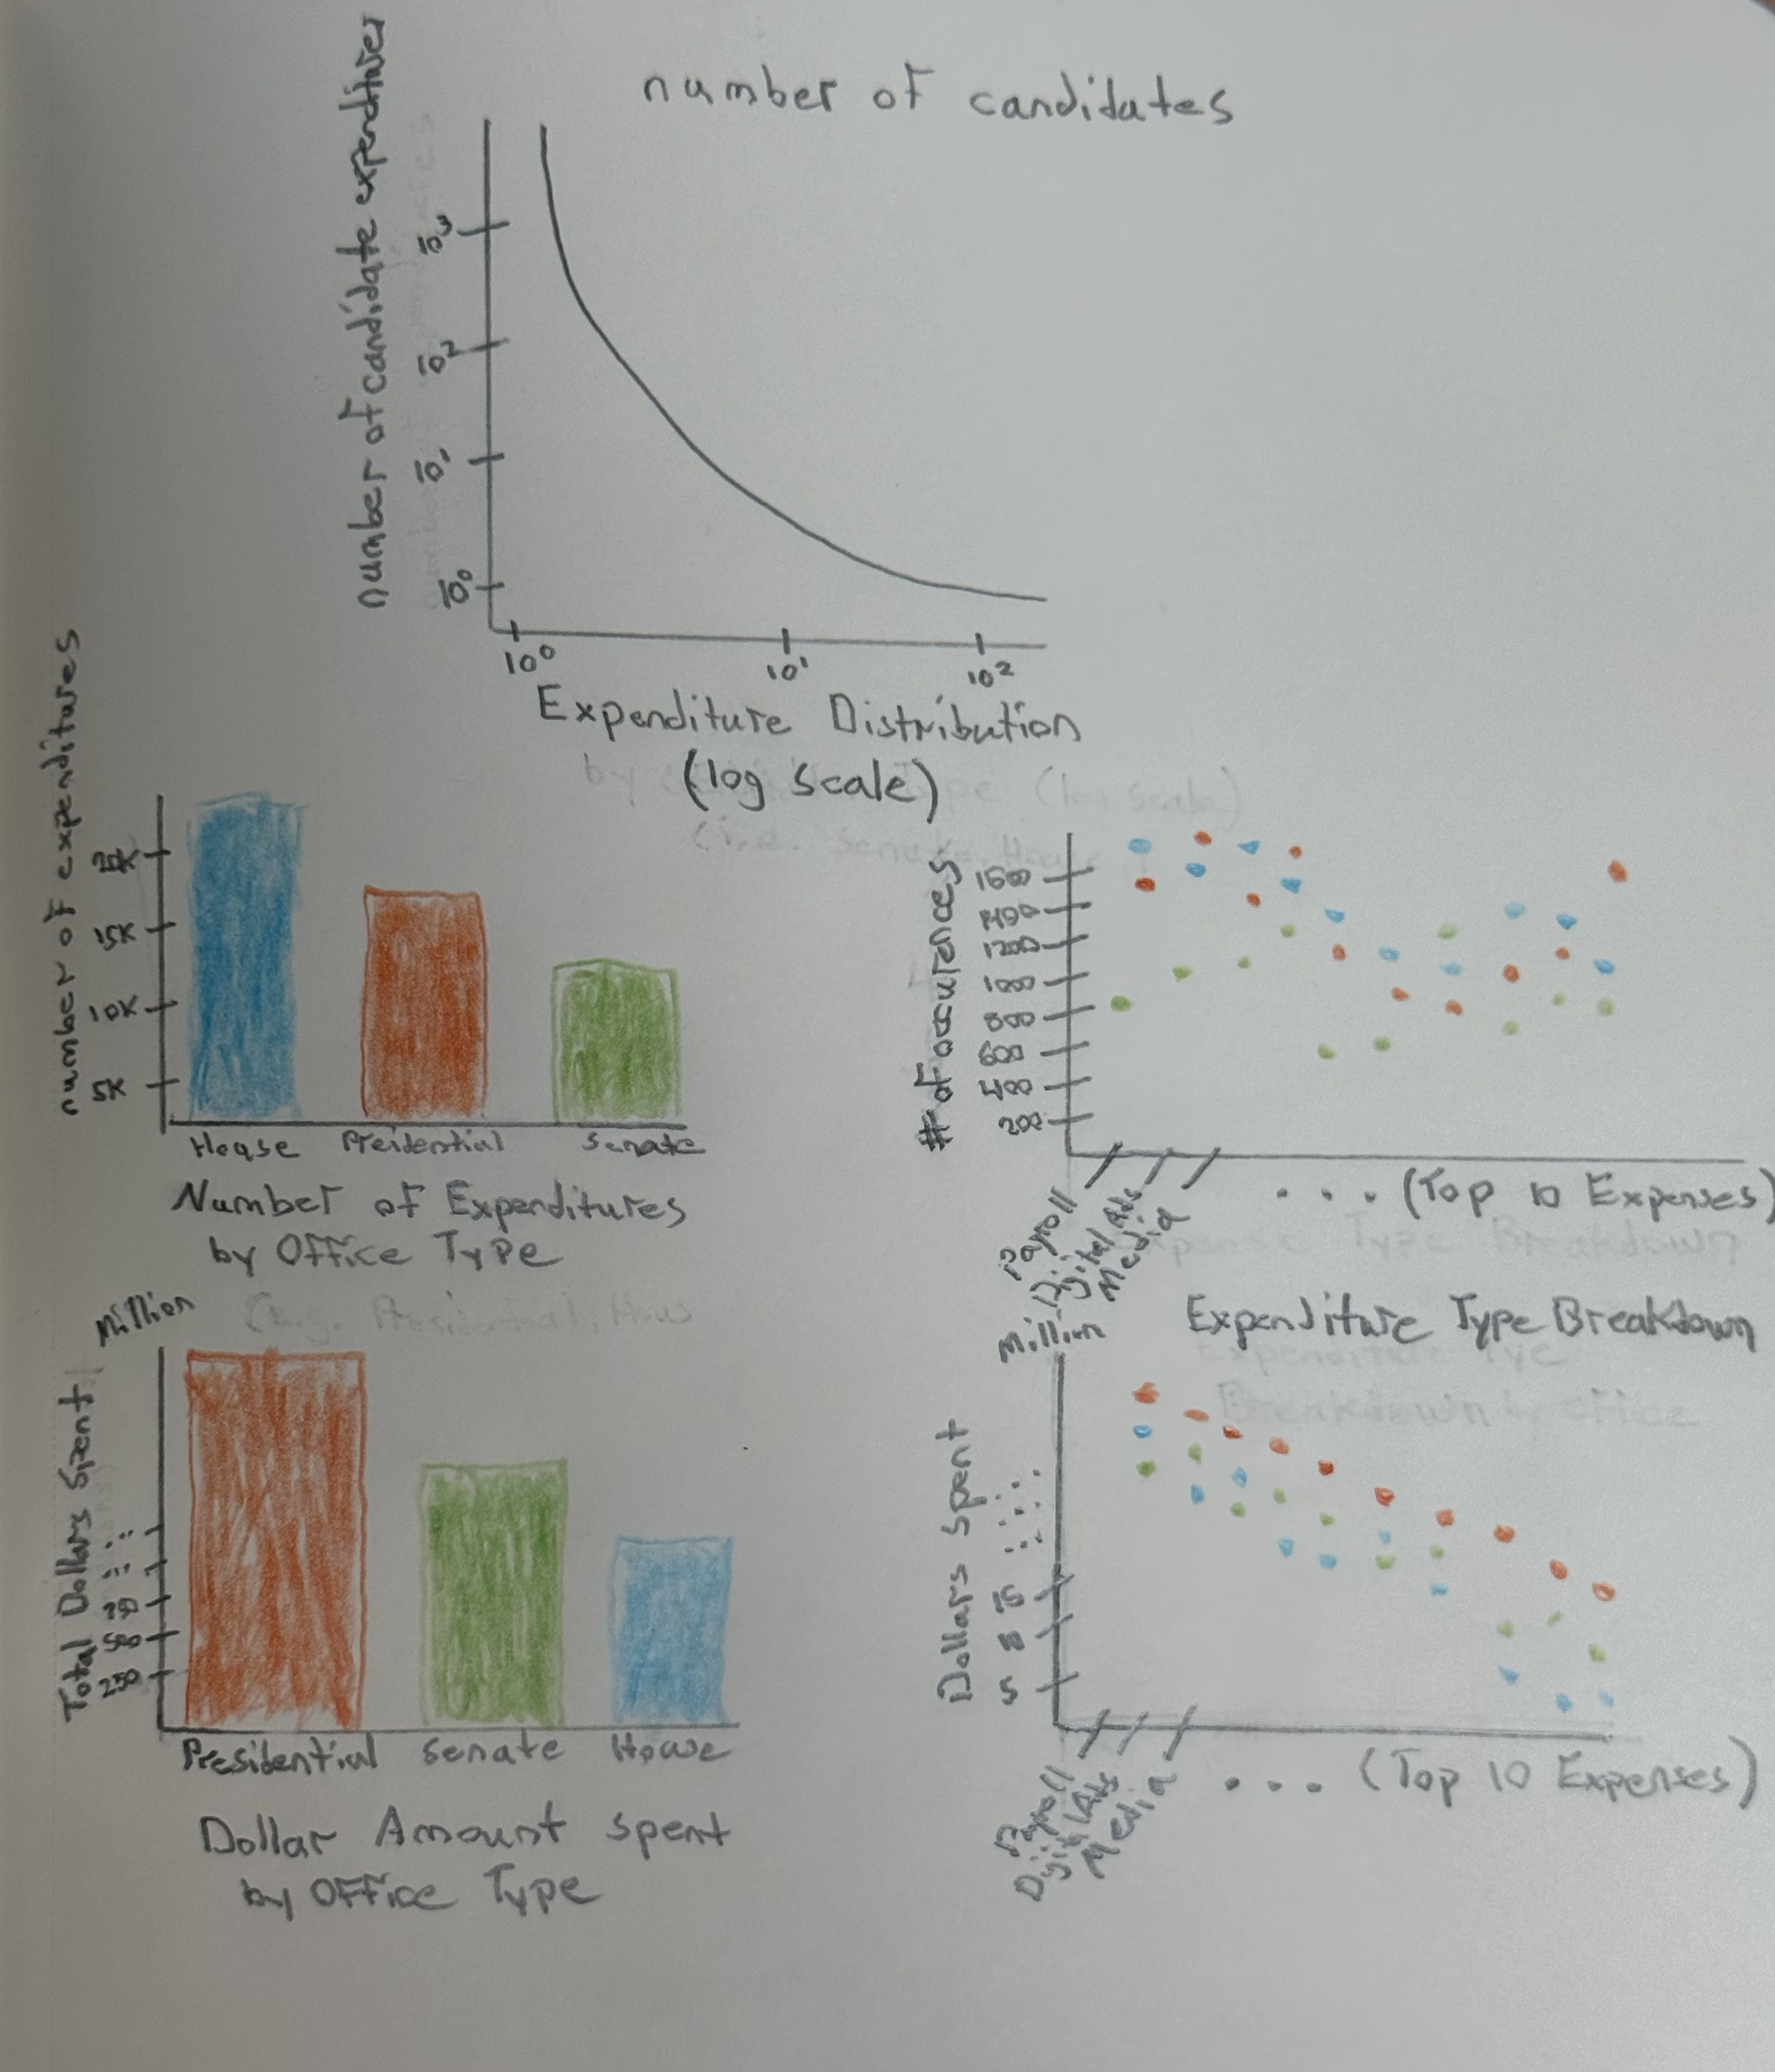
\includegraphics[width=0.8\linewidth]{DS_HW3_hand_drawn.jpeg}
    \caption{A Visually Consistent Plot}
    \label{fig:myfigure}
\end{figure}

In the image above, I start with a cleaner-looking power law distribution by flipping the axis and smoothing out the tail. In the plots below, presented in a top-to-bottom, left-to-right fashion, I begin to unpack and answer the questions that emerged from the provided feedback. First, more context is provided on the expenditure distribution by breaking it down by House, Senate, and Presidential race types. Then the viewer can better understand the actual nature of expenditures through frequency analysis. Finally, we translate expenditures into dollars, following the same narrative structure. Each plot provides a key piece of information that helps tell a bigger story.

What the viewer must keep in mind while interpreting this data is that there were primarily 2 presidential candidates in this dataset, compared to hundreds of House and Senate candidates. As one navigates these visualizations with this context in mind, the true magnitude of presidential elections in this country becomes apparent—not only in terms of money, but in human effort and organizational complexity as well.

\subsection*{Part 2: Translate hand drawn image to plot}

Below there are 3 iterations. The first plot shows a lack of success in the scatter plots due to a lack of consistency across expenditure types.

\begin{figure}[htbp]
    \centering
    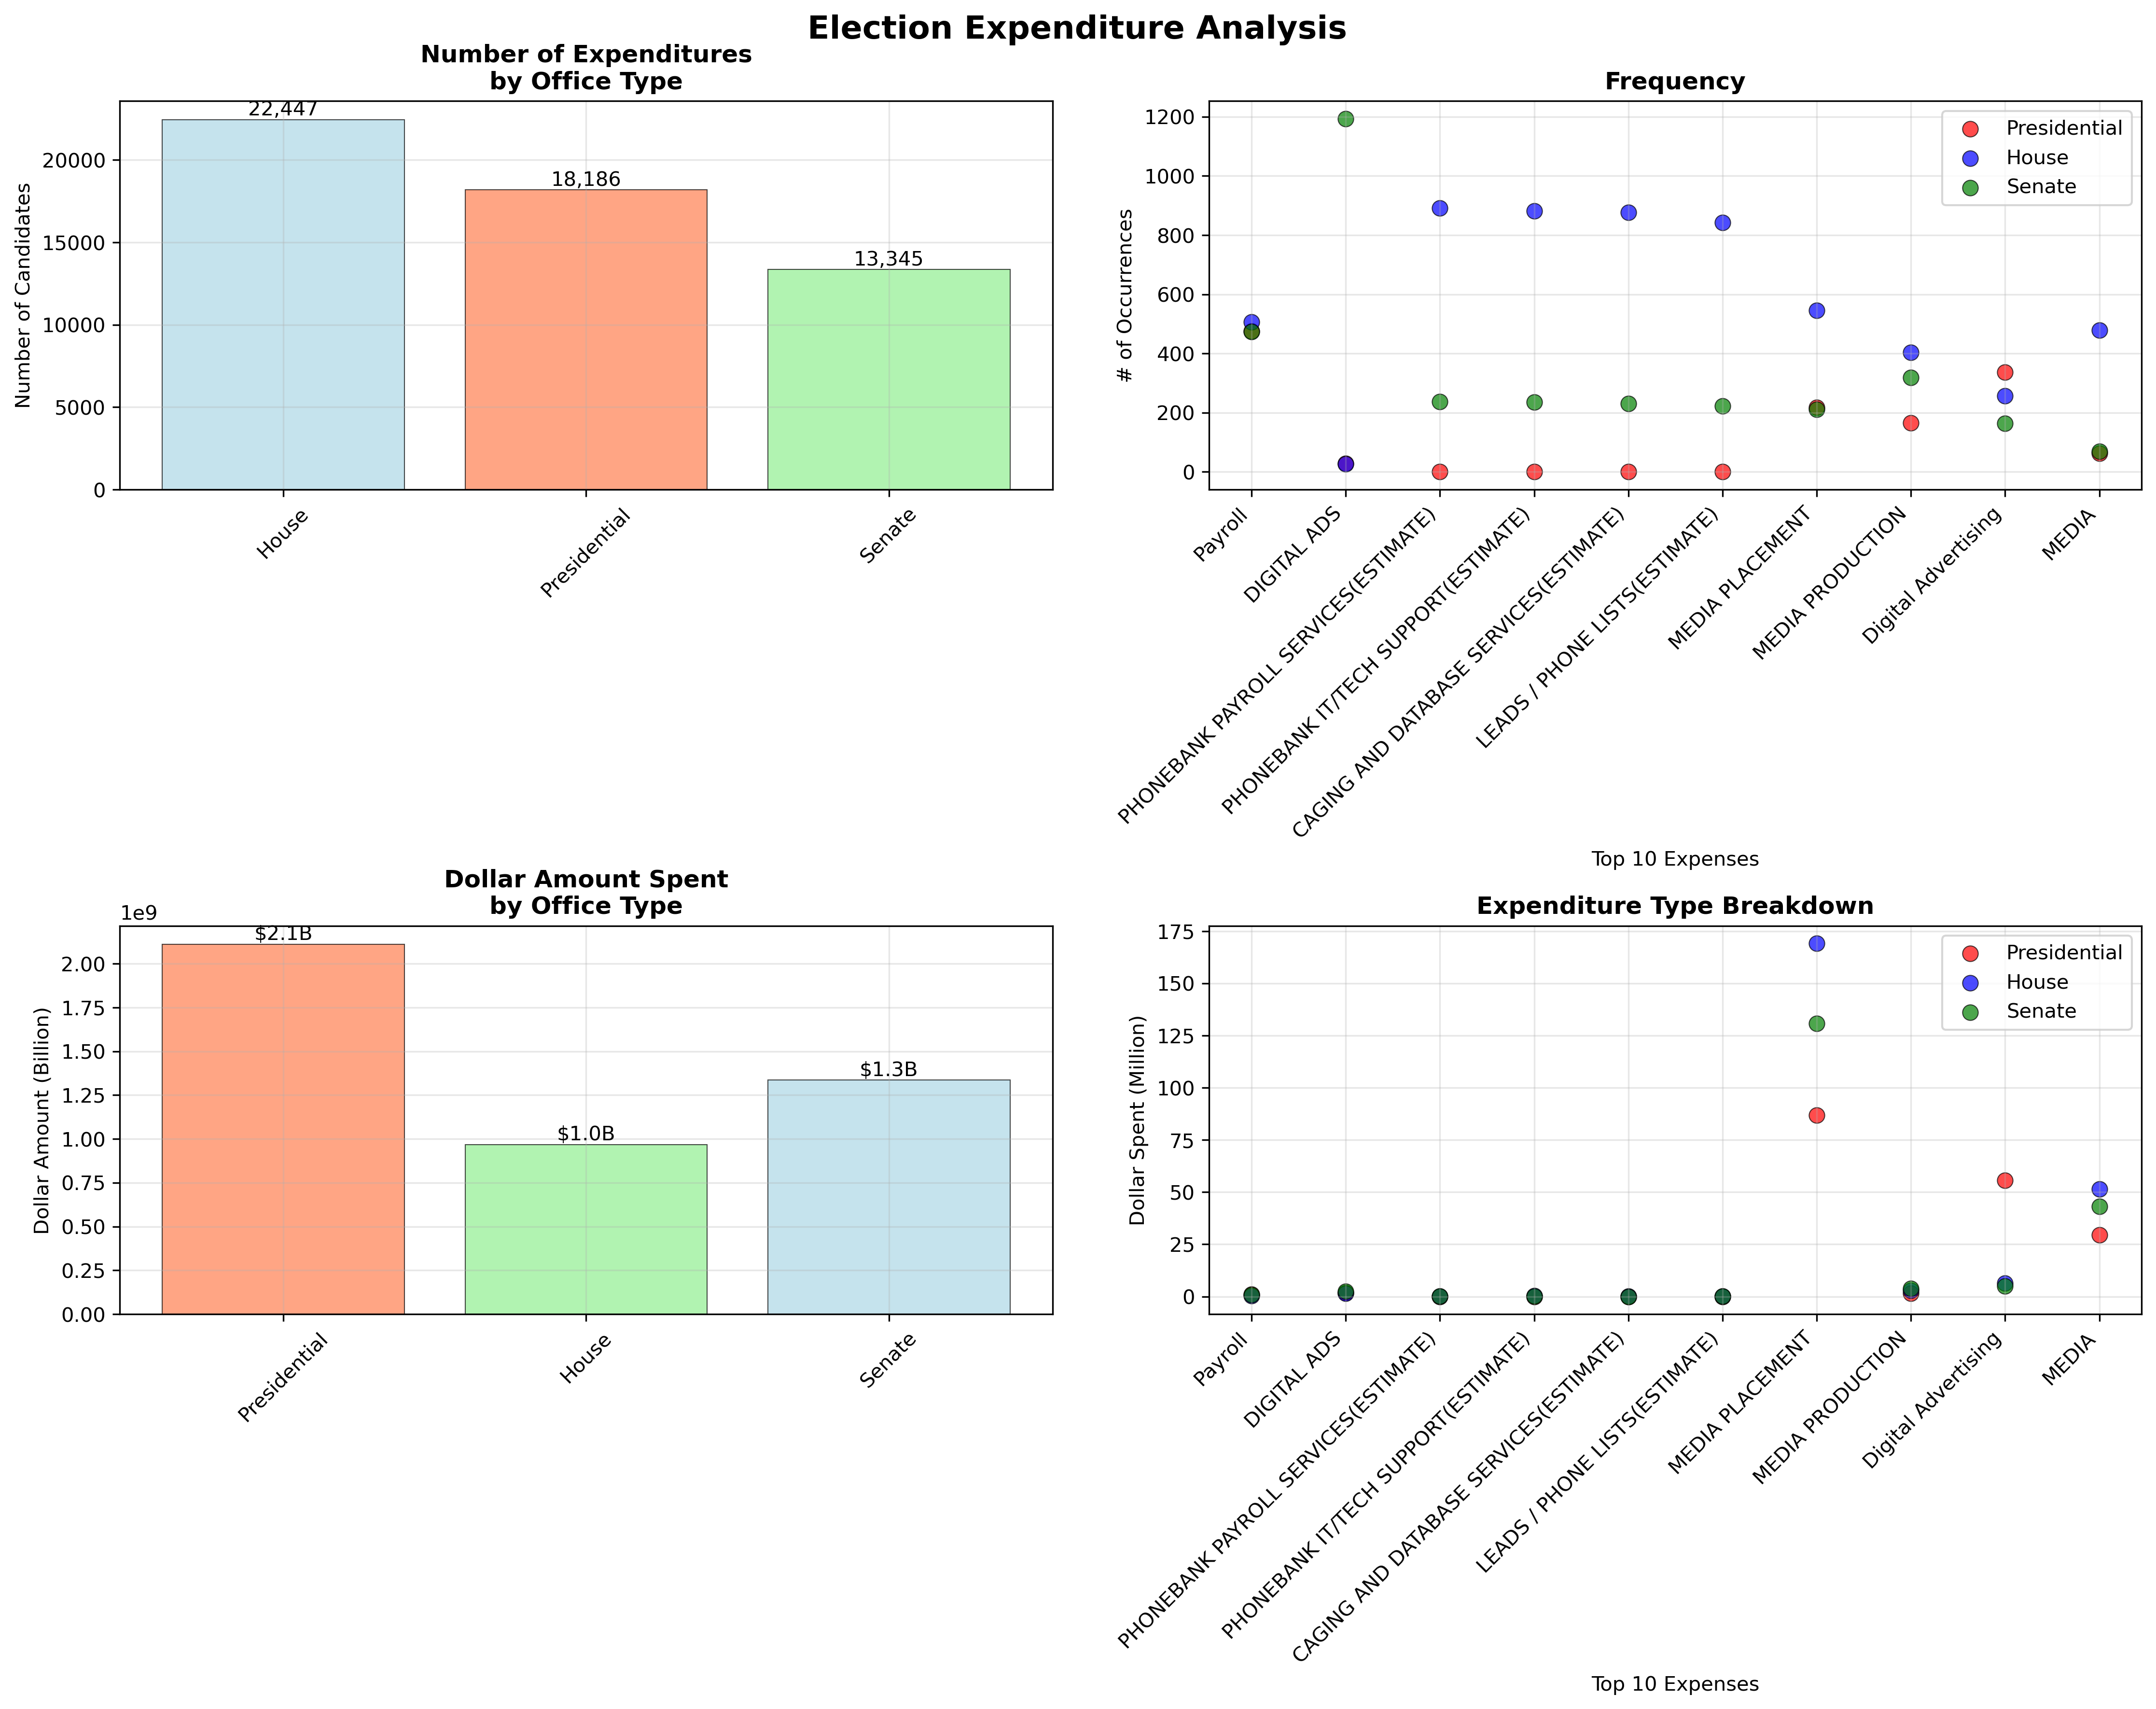
\includegraphics[width=0.8\linewidth]{election_expenditure_analysis_iteration_1.png}
    \caption{Iteration 1}
    \label{fig:myfigure}
\end{figure}

To address the lack of consistency I decided to create horizontal bar plots that displayed spending for presidential and non-presidential (house and senate) office types. The idea being that the flow would go as follows:

expenditure breakdown count by office type -> translate expenditure counts to money spent -> breakdown the way the money is spent by office types

However, I still found this approach a bit confusing, and I felt it didn't address the questions I set out to answer with these plots. Also, I felt that I totally failed to achieve a visually consistent language. What follows is something much nicer!

\begin{figure}[htbp]
    \centering
    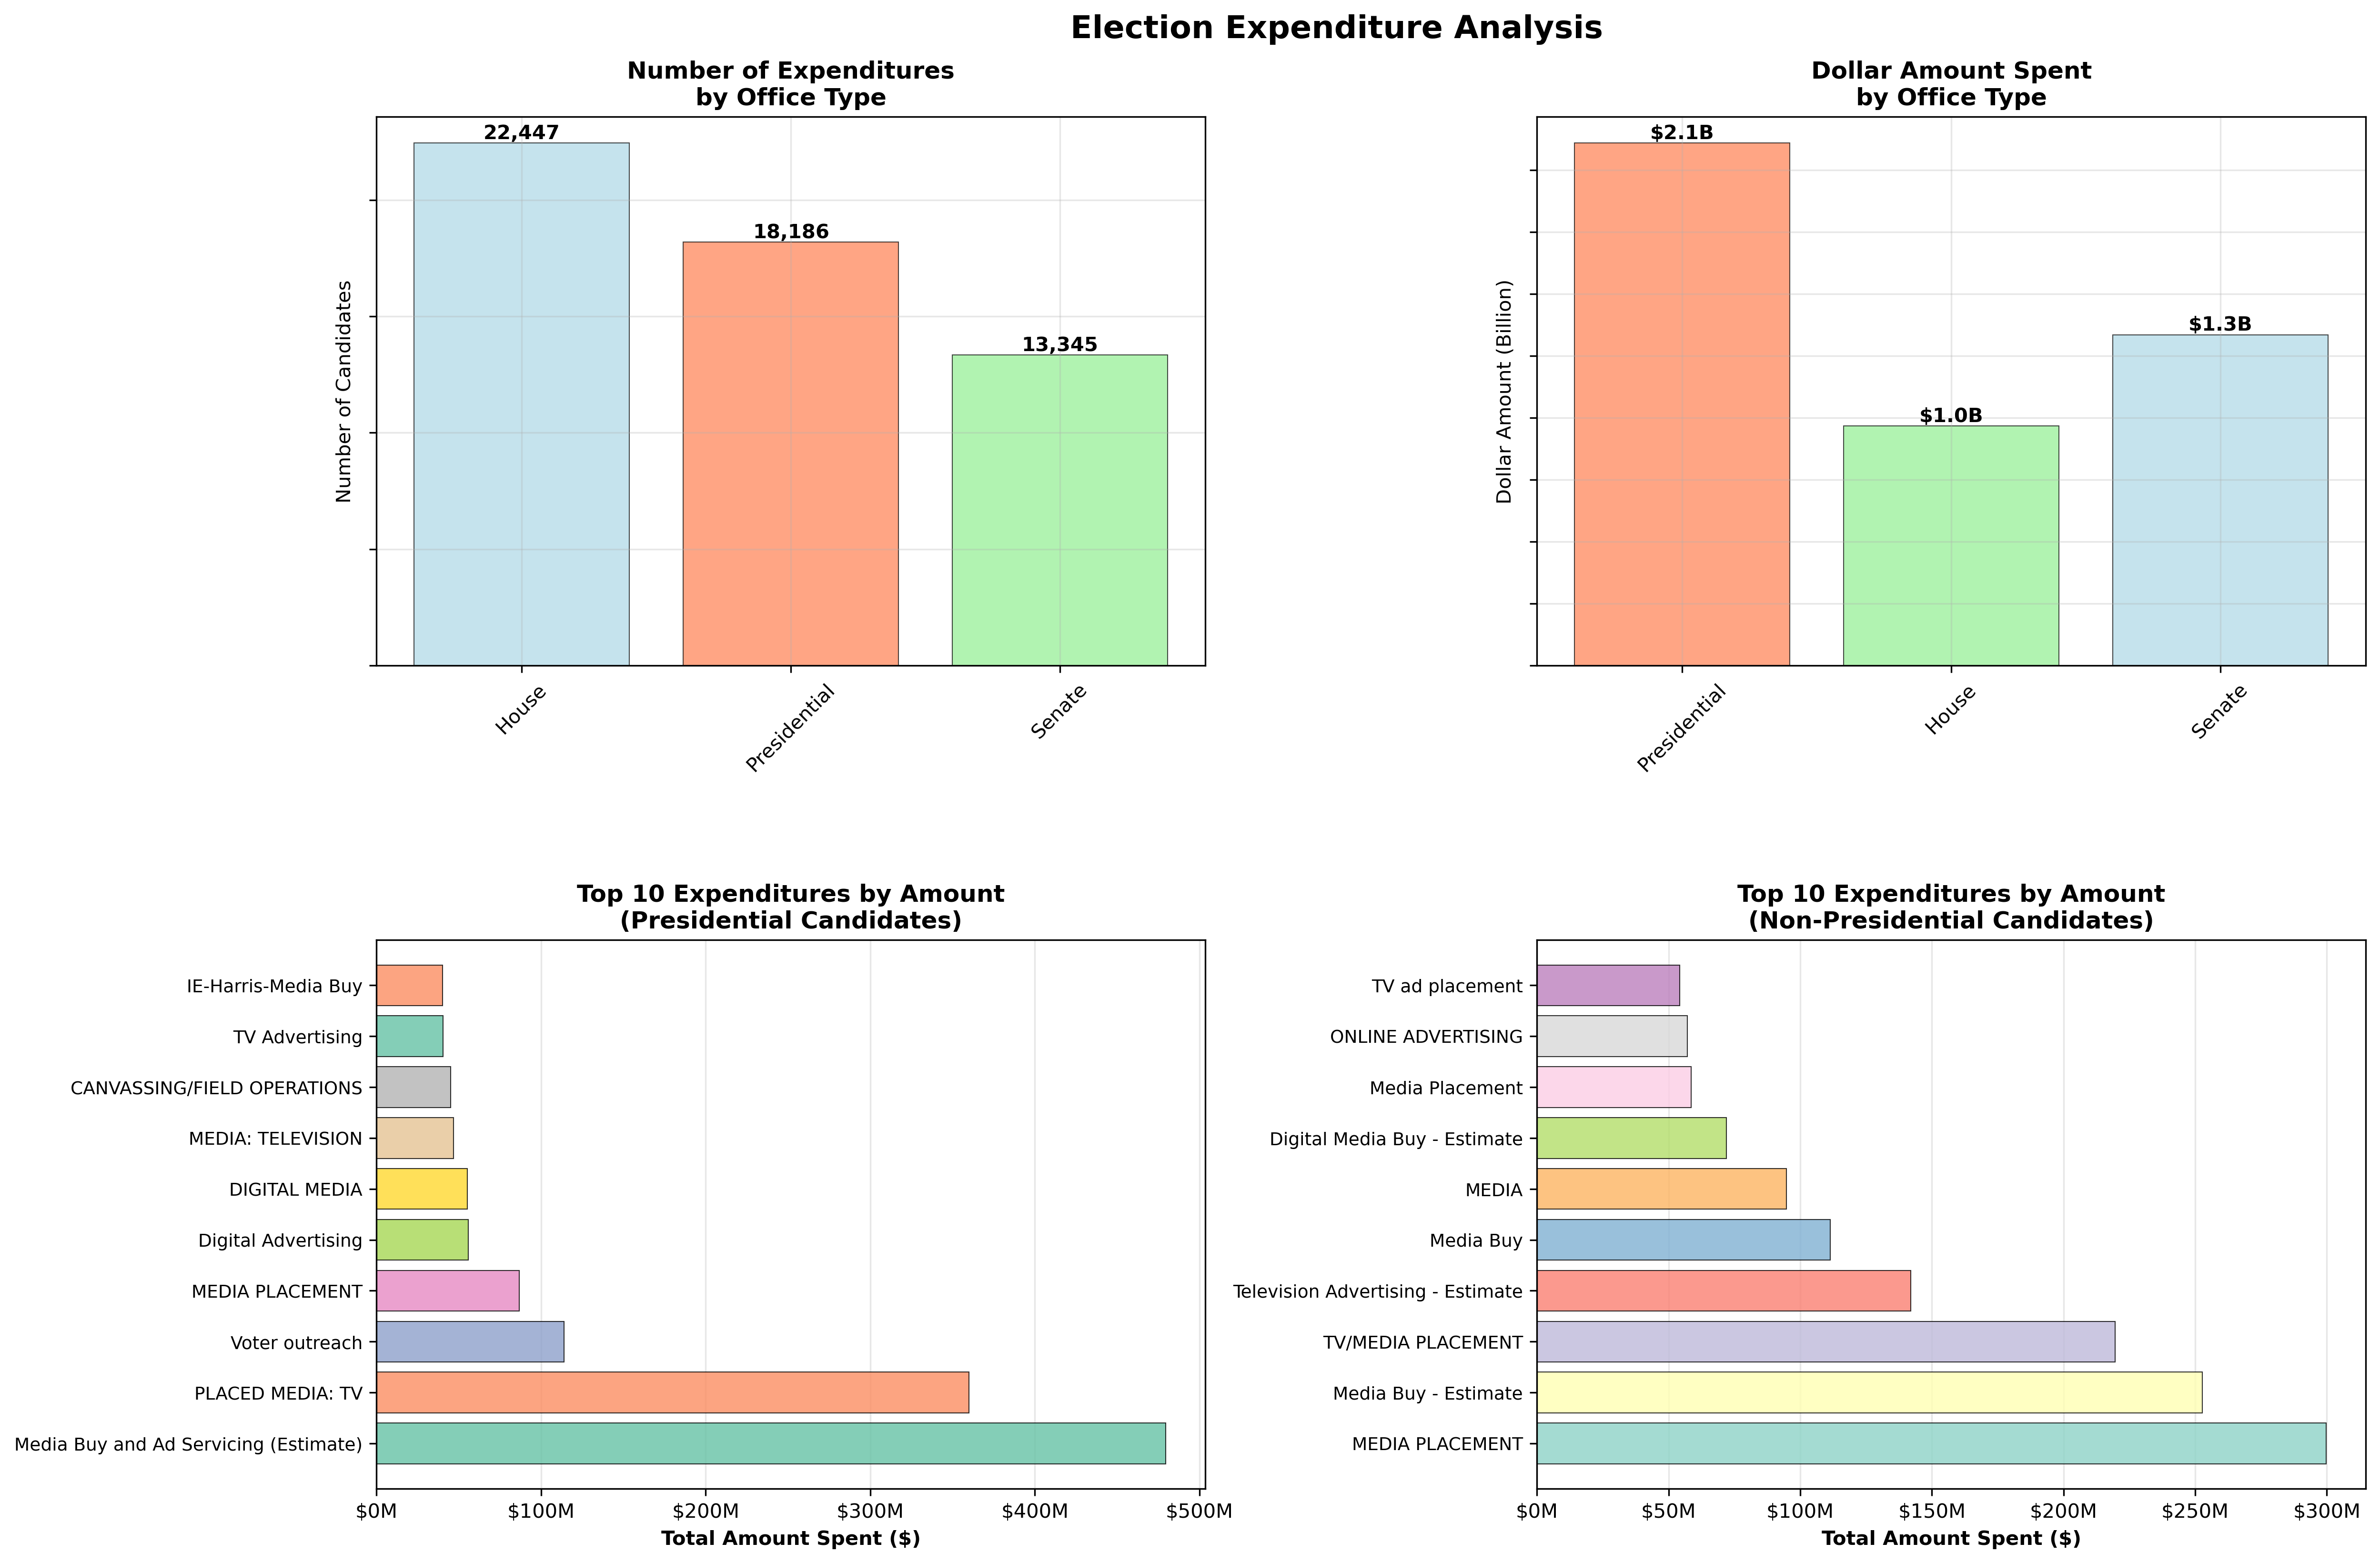
\includegraphics[width=0.8\linewidth]{election_expenditure_analysis_iteration_2.png}
    \caption{Itreation 2}
    \label{fig:myfigure}
\end{figure}

\begin{figure}[H]
    \centering
    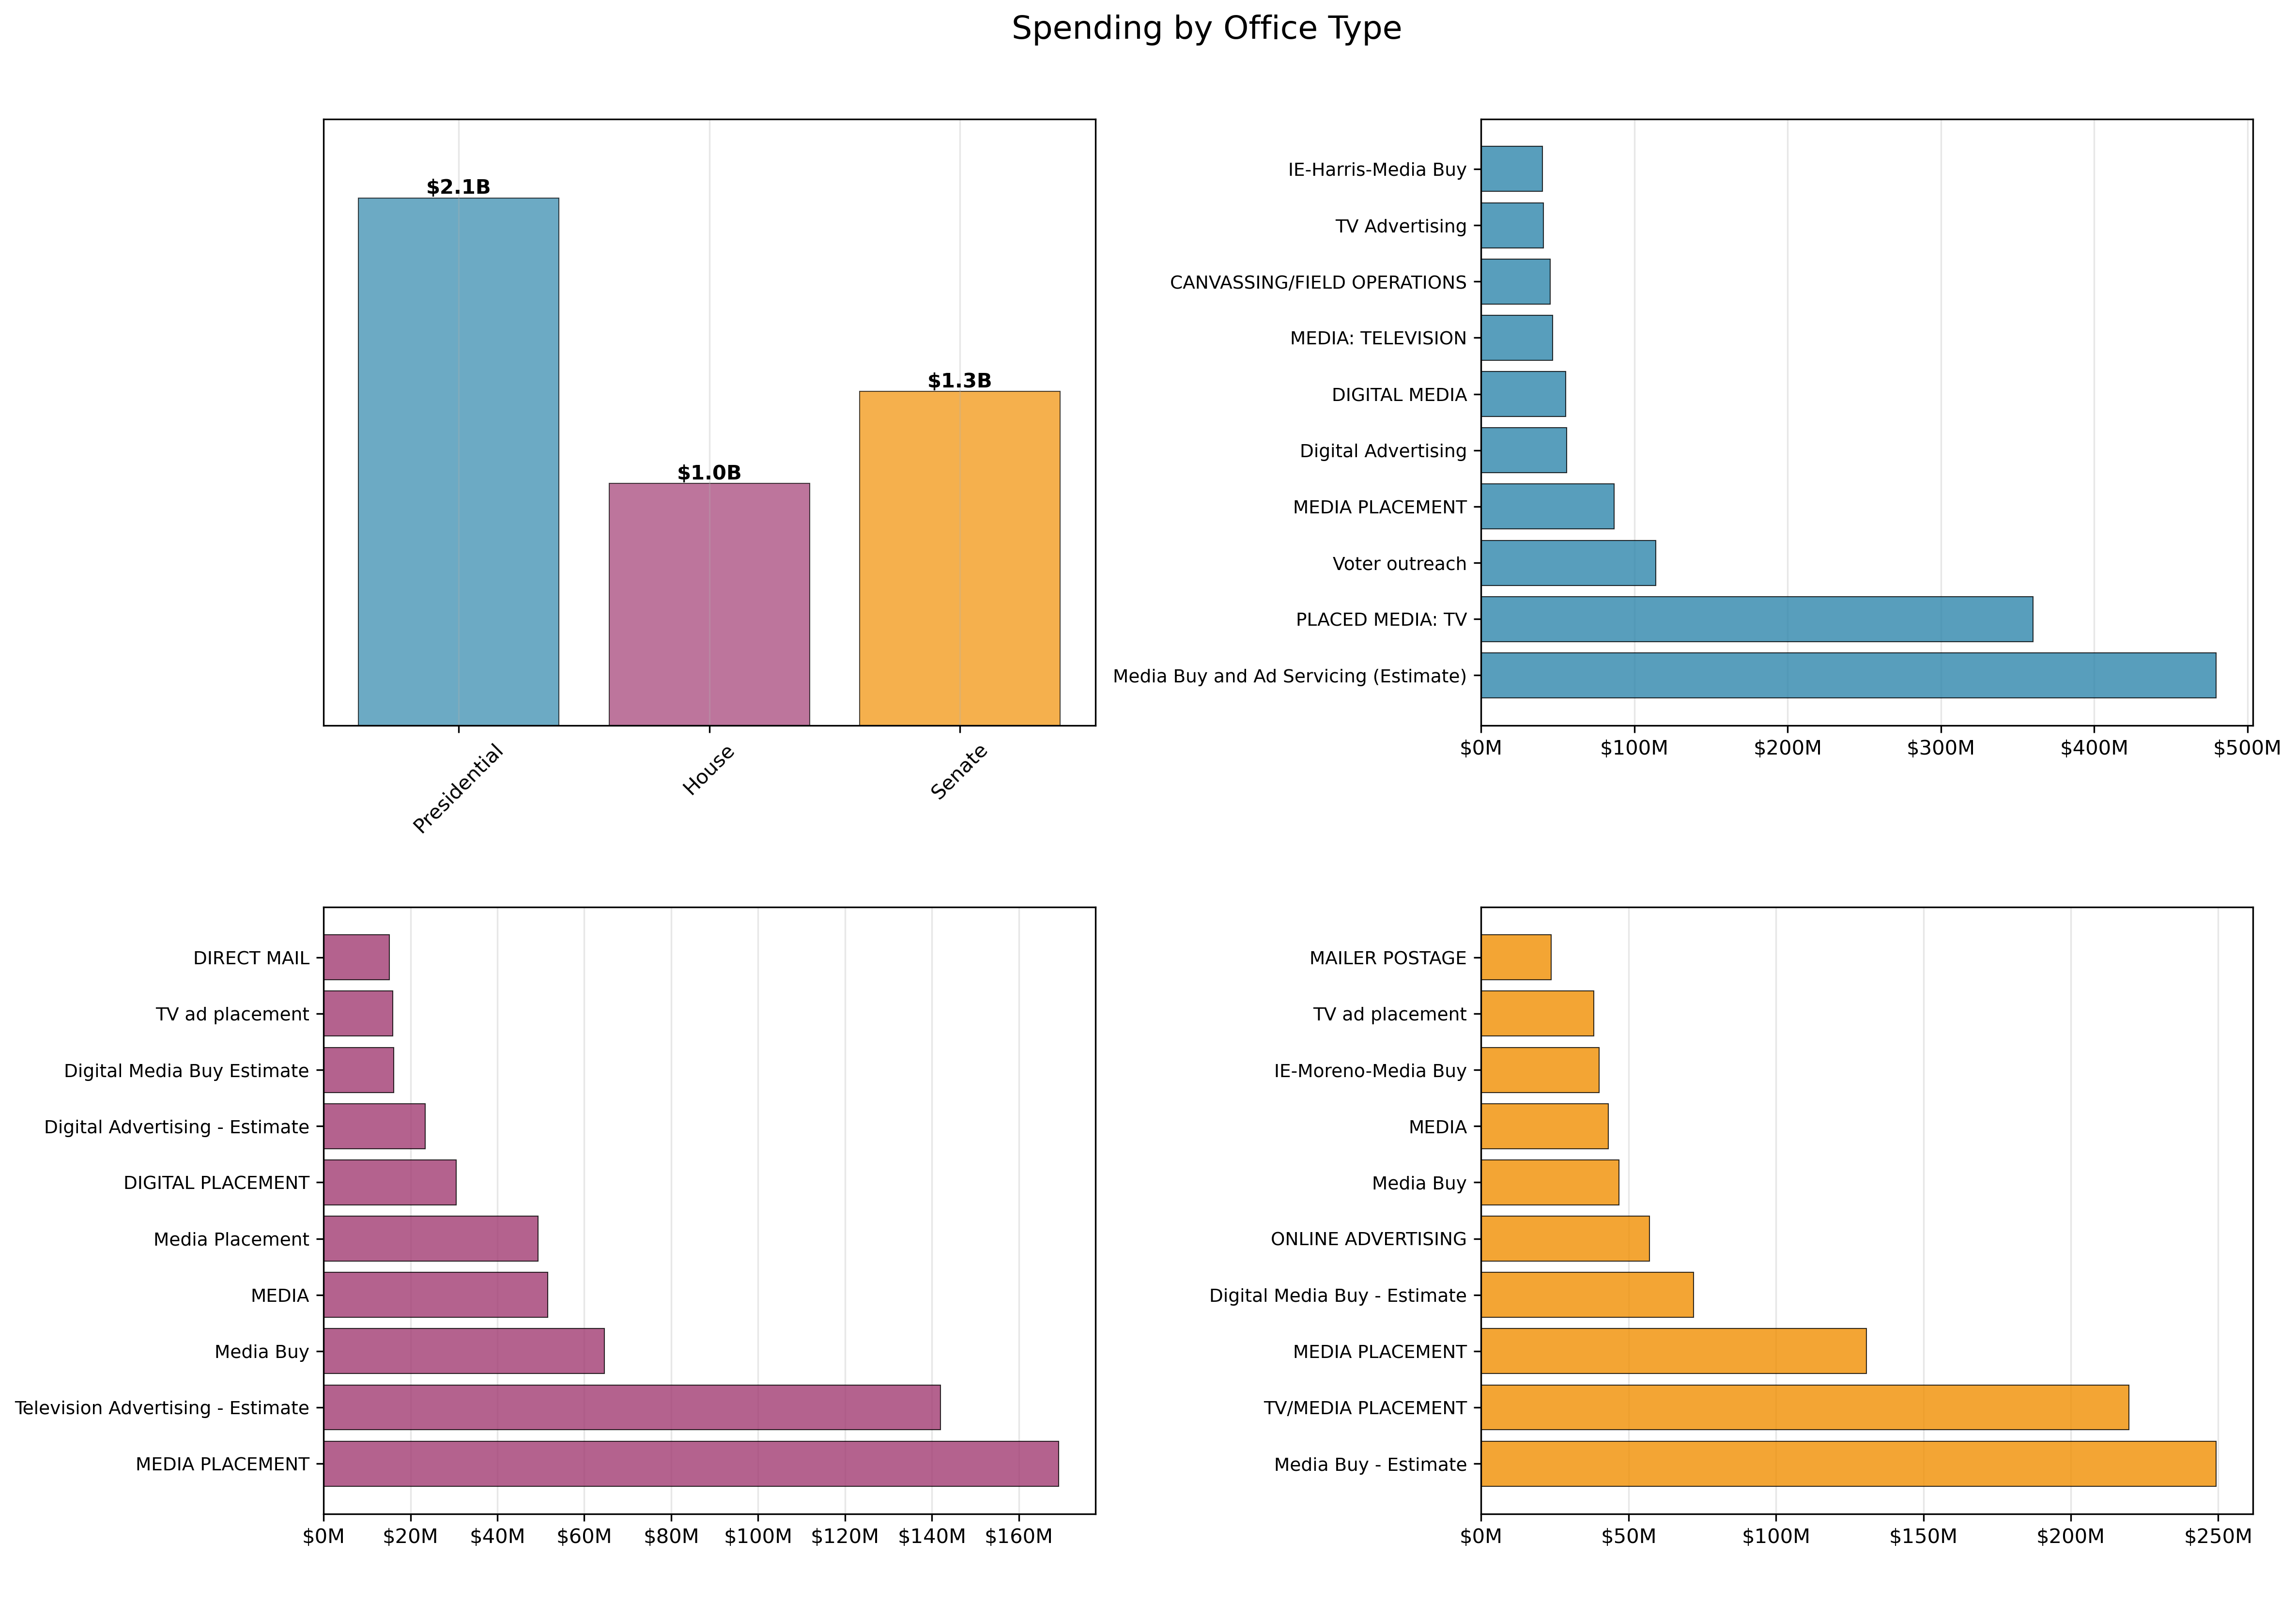
\includegraphics[width=0.8\linewidth]{election_expenditure_analysis_iteration_3.png}
    \caption{Iteration 3}
    \label{fig:myfigure}
\end{figure}

\section*{Question 2: Causal Statements}

\subsection*{Statement 1}

\textbf{Causal Statement:} "There are certain groups of people that don't take vaccines and don't take any pills and have no autism." - Donald Trump

\begin{center}
\begin{tikzcd}
	{\text{Certain Groups}} & {\text{No Vaccines}} \\
	{\text{No Pills}} & {\text{No Autism}}
	\arrow[dotted, from=1-1, to=1-2]
	\arrow[dotted, from=1-1, to=2-1]
	\arrow[from=1-2, to=2-2]
	\arrow[from=2-1, to=2-2]
\end{tikzcd}
\end{center}

\subsubsection*{Analysis Questions:}

\textbf{Counterfactual:}

The implicit counterfactual here is that if certain groups (e.g. "The Amish") vaccinated and took pills, they would have autism in their population.

\vspace{0.5in}
\textbf{Ideal Experiment:}

An ideal experiment here would be to research communities where access to Tylenol and vaccines is limited by socioeconomic circumstances rather than a belief system. This kind of experiment would be generational and track groups that engaged with Tylenol, vaccines, both as well as a control group.

\vspace{0.5in}
\textbf{Potential Confounds:}
\begin{itemize}
    \item Socioeconomic status: Wealthier families may be more likely to both avoid vaccines AND have better access to early autism diagnosis/services
    \item Education/beliefs: Parents who avoid vaccines may also avoid seeking autism diagnoses due to stigma or distrust of medical establishment
\end{itemize}
\vspace{0.5in}

\subsection*{Statement 2}

\textbf{Causal Statement:} Democrats are about to shutdown the government because they demand we fund healthcare for illegal aliens." - JD Vance

\begin{center}
\[\begin{tikzcd}
	& {\text{Democrats}} \\
	& {\text{fund healthcare}} \\
	{\text{non-citizens}} && {\text{citizens}} \\
	& {\text{government shutdown}} && {\text{government does not shutdown}} \\
	&& {\text{loss of essential services for all}}
	\arrow[from=1-2, to=2-2]
	\arrow[from=2-2, to=3-1]
	\arrow[from=2-2, to=3-3]
	\arrow[from=3-1, to=4-2]
	\arrow[from=3-3, to=4-4]
	\arrow[from=4-2, to=5-3]
\end{tikzcd}\]
\end{center}

\subsubsection{Analysis Questions:}

\textbf{Counterfactual:}

The reverse implication of this statement would be that Democrats do not fund healthcare for non-citizens and the government stays open.

\vspace{0.5in}

\textbf{Potential Confounds:}
\begin{itemize}
    \item Budget negotiations complexity: A shutdown might ultimately occur due to a failure to negotiate a multitude of complex issues. Publ 
    \item Public opinion: This may be an effort to pressure Democrats to cave by controlling the narrative.
    \item Distraction: This could be an effort to distract from actual healthcare funding disputes (Medicare, Medicaid, ACA tax credits).
\end{itemize}

\vspace{0.5in}

\subsection*{Statement 3}

\textbf{Causal Statement:} "Marvel is better than DC because they have less stereotypical superhero ideas like The Thing versus Superman. The Thing's powers can impede him. They stop him from living a normal life because of his rock-like skin and monstrous appearance, but Superman has all the benefits of being a superhero - speed, superhuman strength, but none of the downsides."

\begin{center}
\begin{tikzcd}
	{\text{Superheros}} & {\text{Flaws}} & {\text{Character Depth}} & {\text{Story Quality}} \\
	{\text{The Thing - Marvel}} & {\text{rock-like skin and monstrous appearance}} & {\text{Complex character}} & {\text{Better}} \\
	{\text{Superman - DC}} & {\text{No apparent flaws}} & {\text{Simpler character}} & {\text{Worse}}
	\arrow[from=1-1, to=1-2]
	\arrow[from=1-1, to=2-1]
	\arrow[from=1-2, to=1-3]
	\arrow[from=1-3, to=1-4]
	\arrow[from=2-1, to=2-2]
	\arrow[from=2-2, to=2-3]
	\arrow[from=2-3, to=2-4]
	\arrow[from=3-1, to=3-2]
	\arrow[from=3-2, to=3-3]
	\arrow[from=3-3, to=3-4]
\end{tikzcd}
\end{center}

\subsubsection*{Analysis Questions:}\documentclass[12pt]{article}
\usepackage[margin=1in]{geometry}
\usepackage{amsmath}
\usepackage{amsfonts}
\usepackage{amssymb}
\usepackage{tikz-cd}
\usepackage{quiver}
\usepackage{enumitem}
\usepackage{hyperref}

\title{Data Science 1 - HW 3}
\author{CSYS 5870, Fall 2025}
\date{September 26, 2025}

\begin{document}

\maketitle

\section*{Question 1: Revisiting a Previous Visualization}
\subsection*{Part 1: Constructing a hand drawn image}

\begin{figure}[htbp]
    \centering
    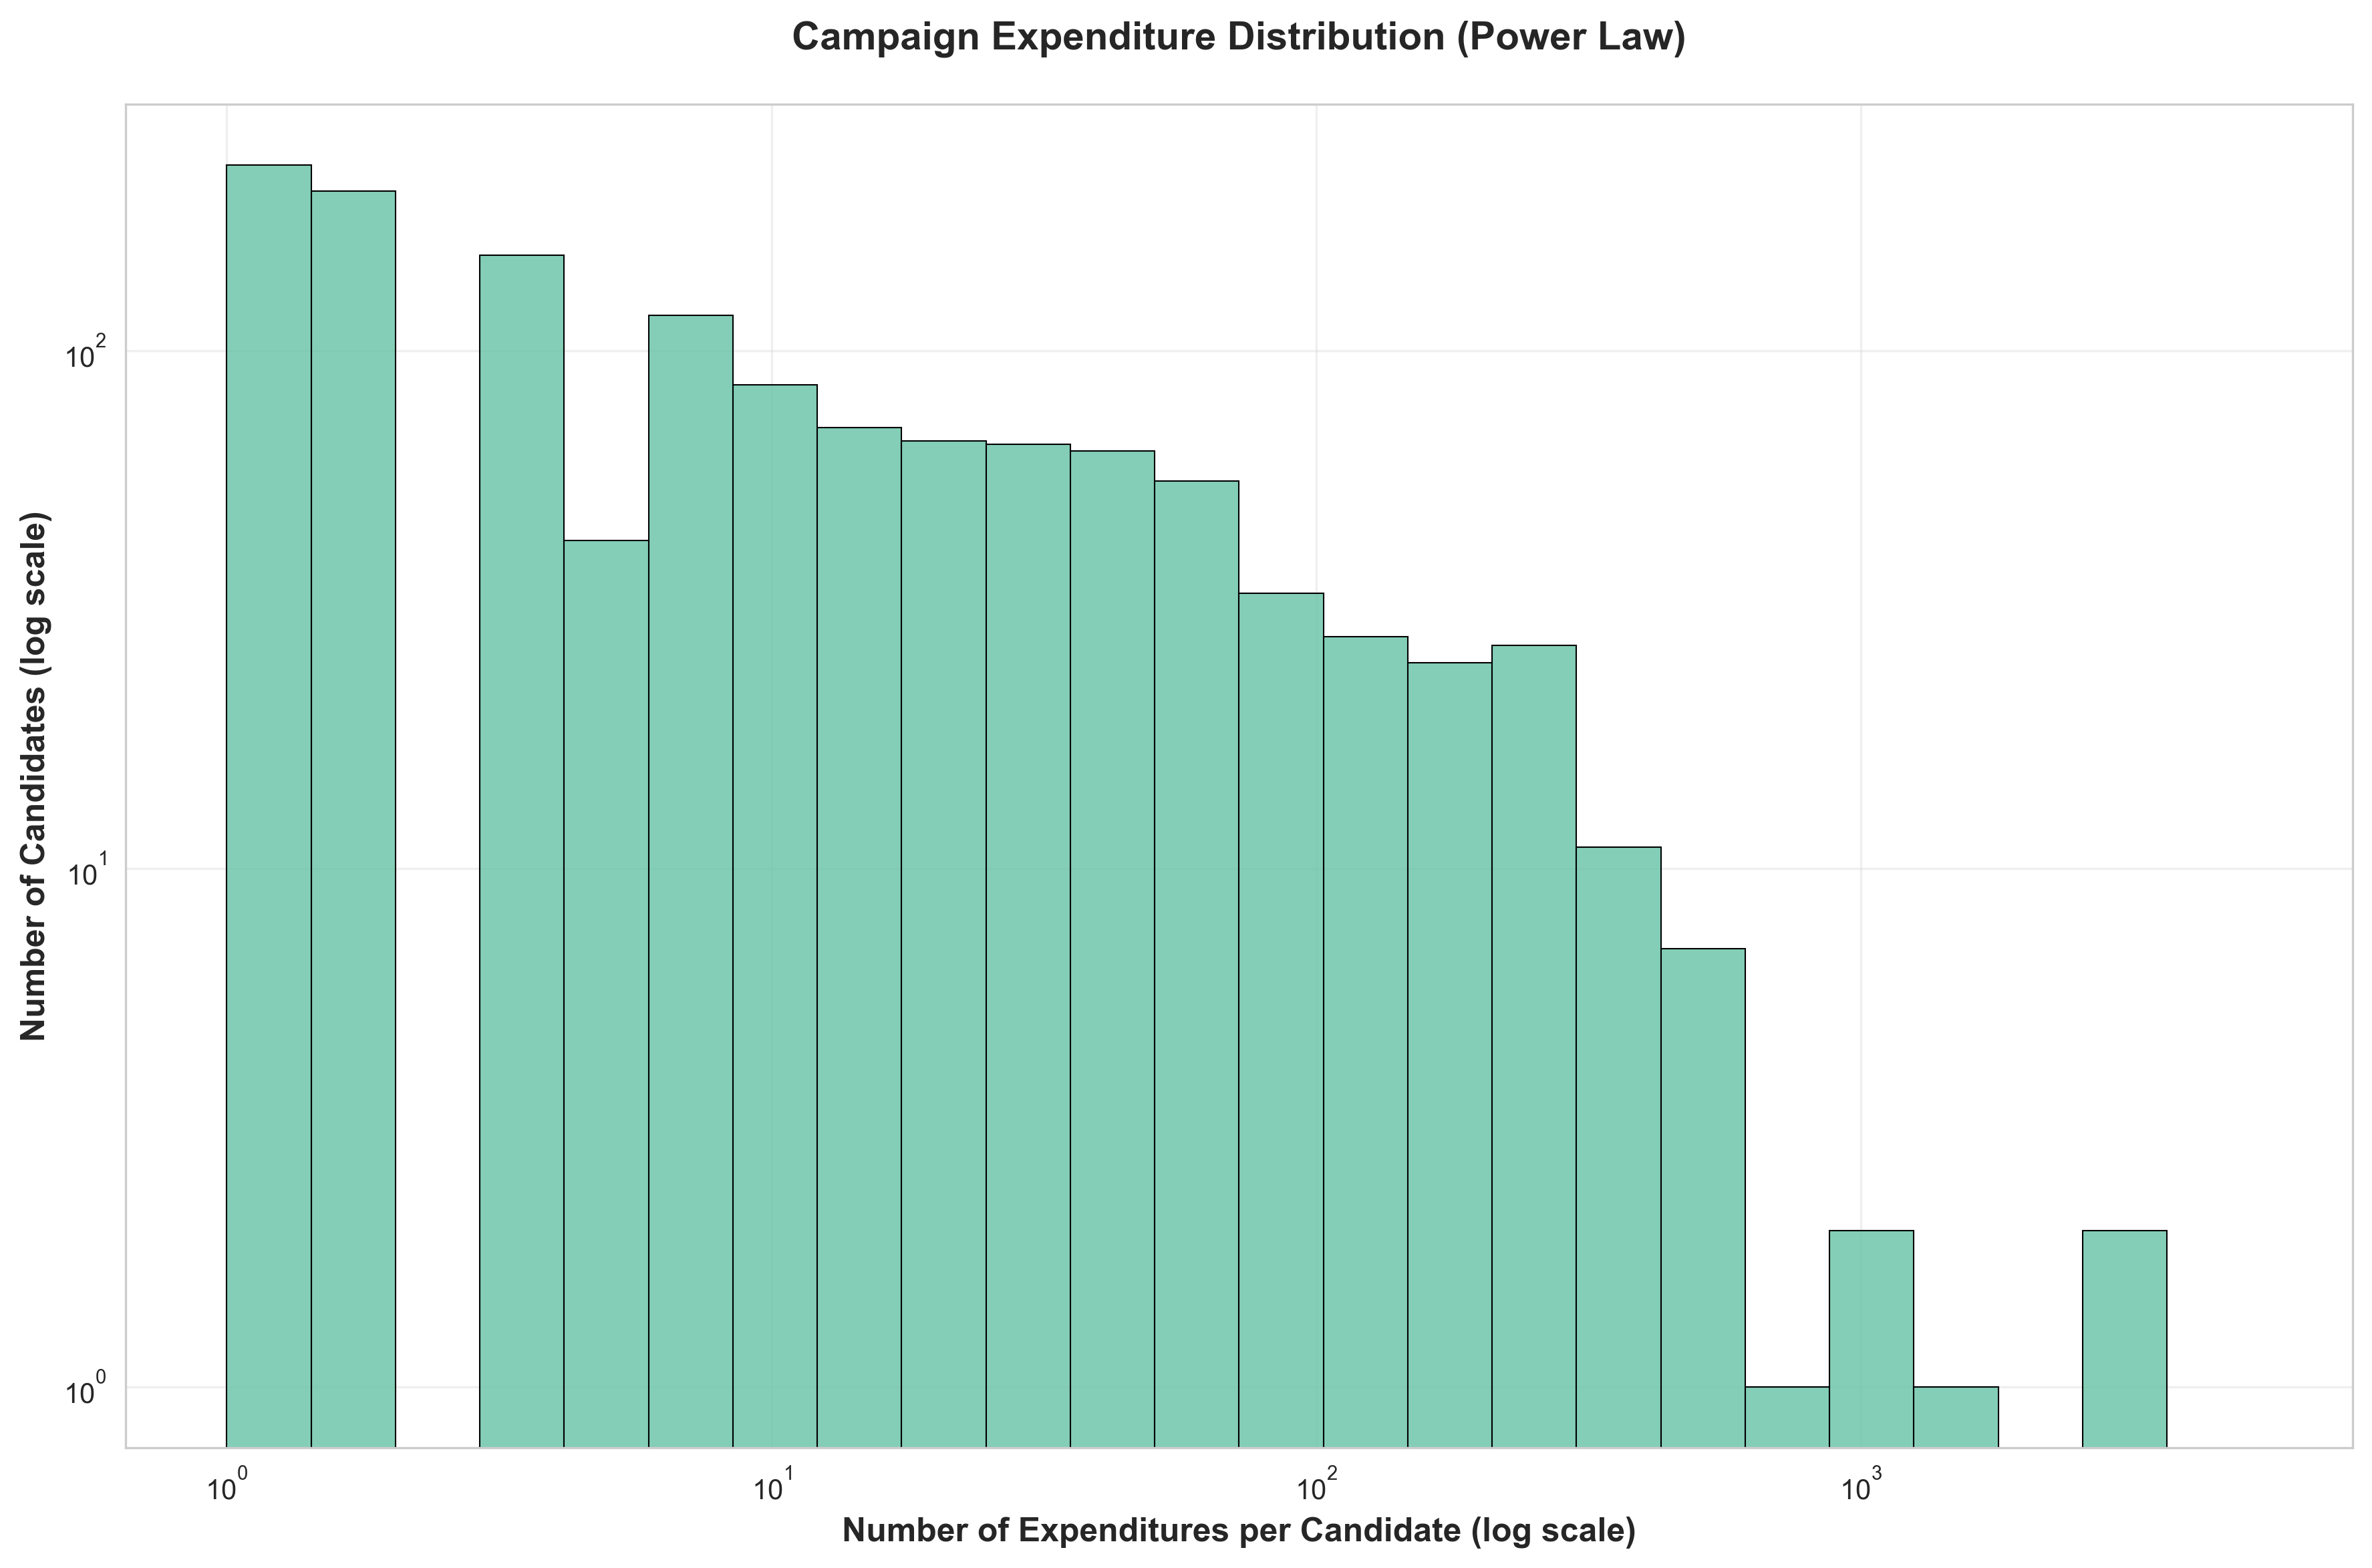
\includegraphics[width=0.8\linewidth]{power_law.png}
    \caption{Image selected to revisit}
    \label{fig:myfigure}
\end{figure}

This plot was an attempt at conveying the idea that campaign expenditures are dominated by 2 individuals. The feedback I received is that the image is confusing. "Perhaps you should flip the axis." The idea was that the tail would be more defined. The bigger question was around the "so what?". 

\begin{itemize}
    \item Why is this distribution important?
    \item What is an expenditure?
    \item How do these expenditures breakdown across candidate/election type?
    \item How do expenditures translate to dollars spent?
    \item How can we visualize how dollars are spent on different types of expenditures?
\end{itemize}

In trying to answer these questions with a hand drawn picture, I tried to focus on how a visualization might flow from panel to panel. My inspiration came from Claus Wilke's "compound figures" - specifically I tried to "employ a consistent visual language" in telling my story.

\begin{figure}[htbp]
    \centering
    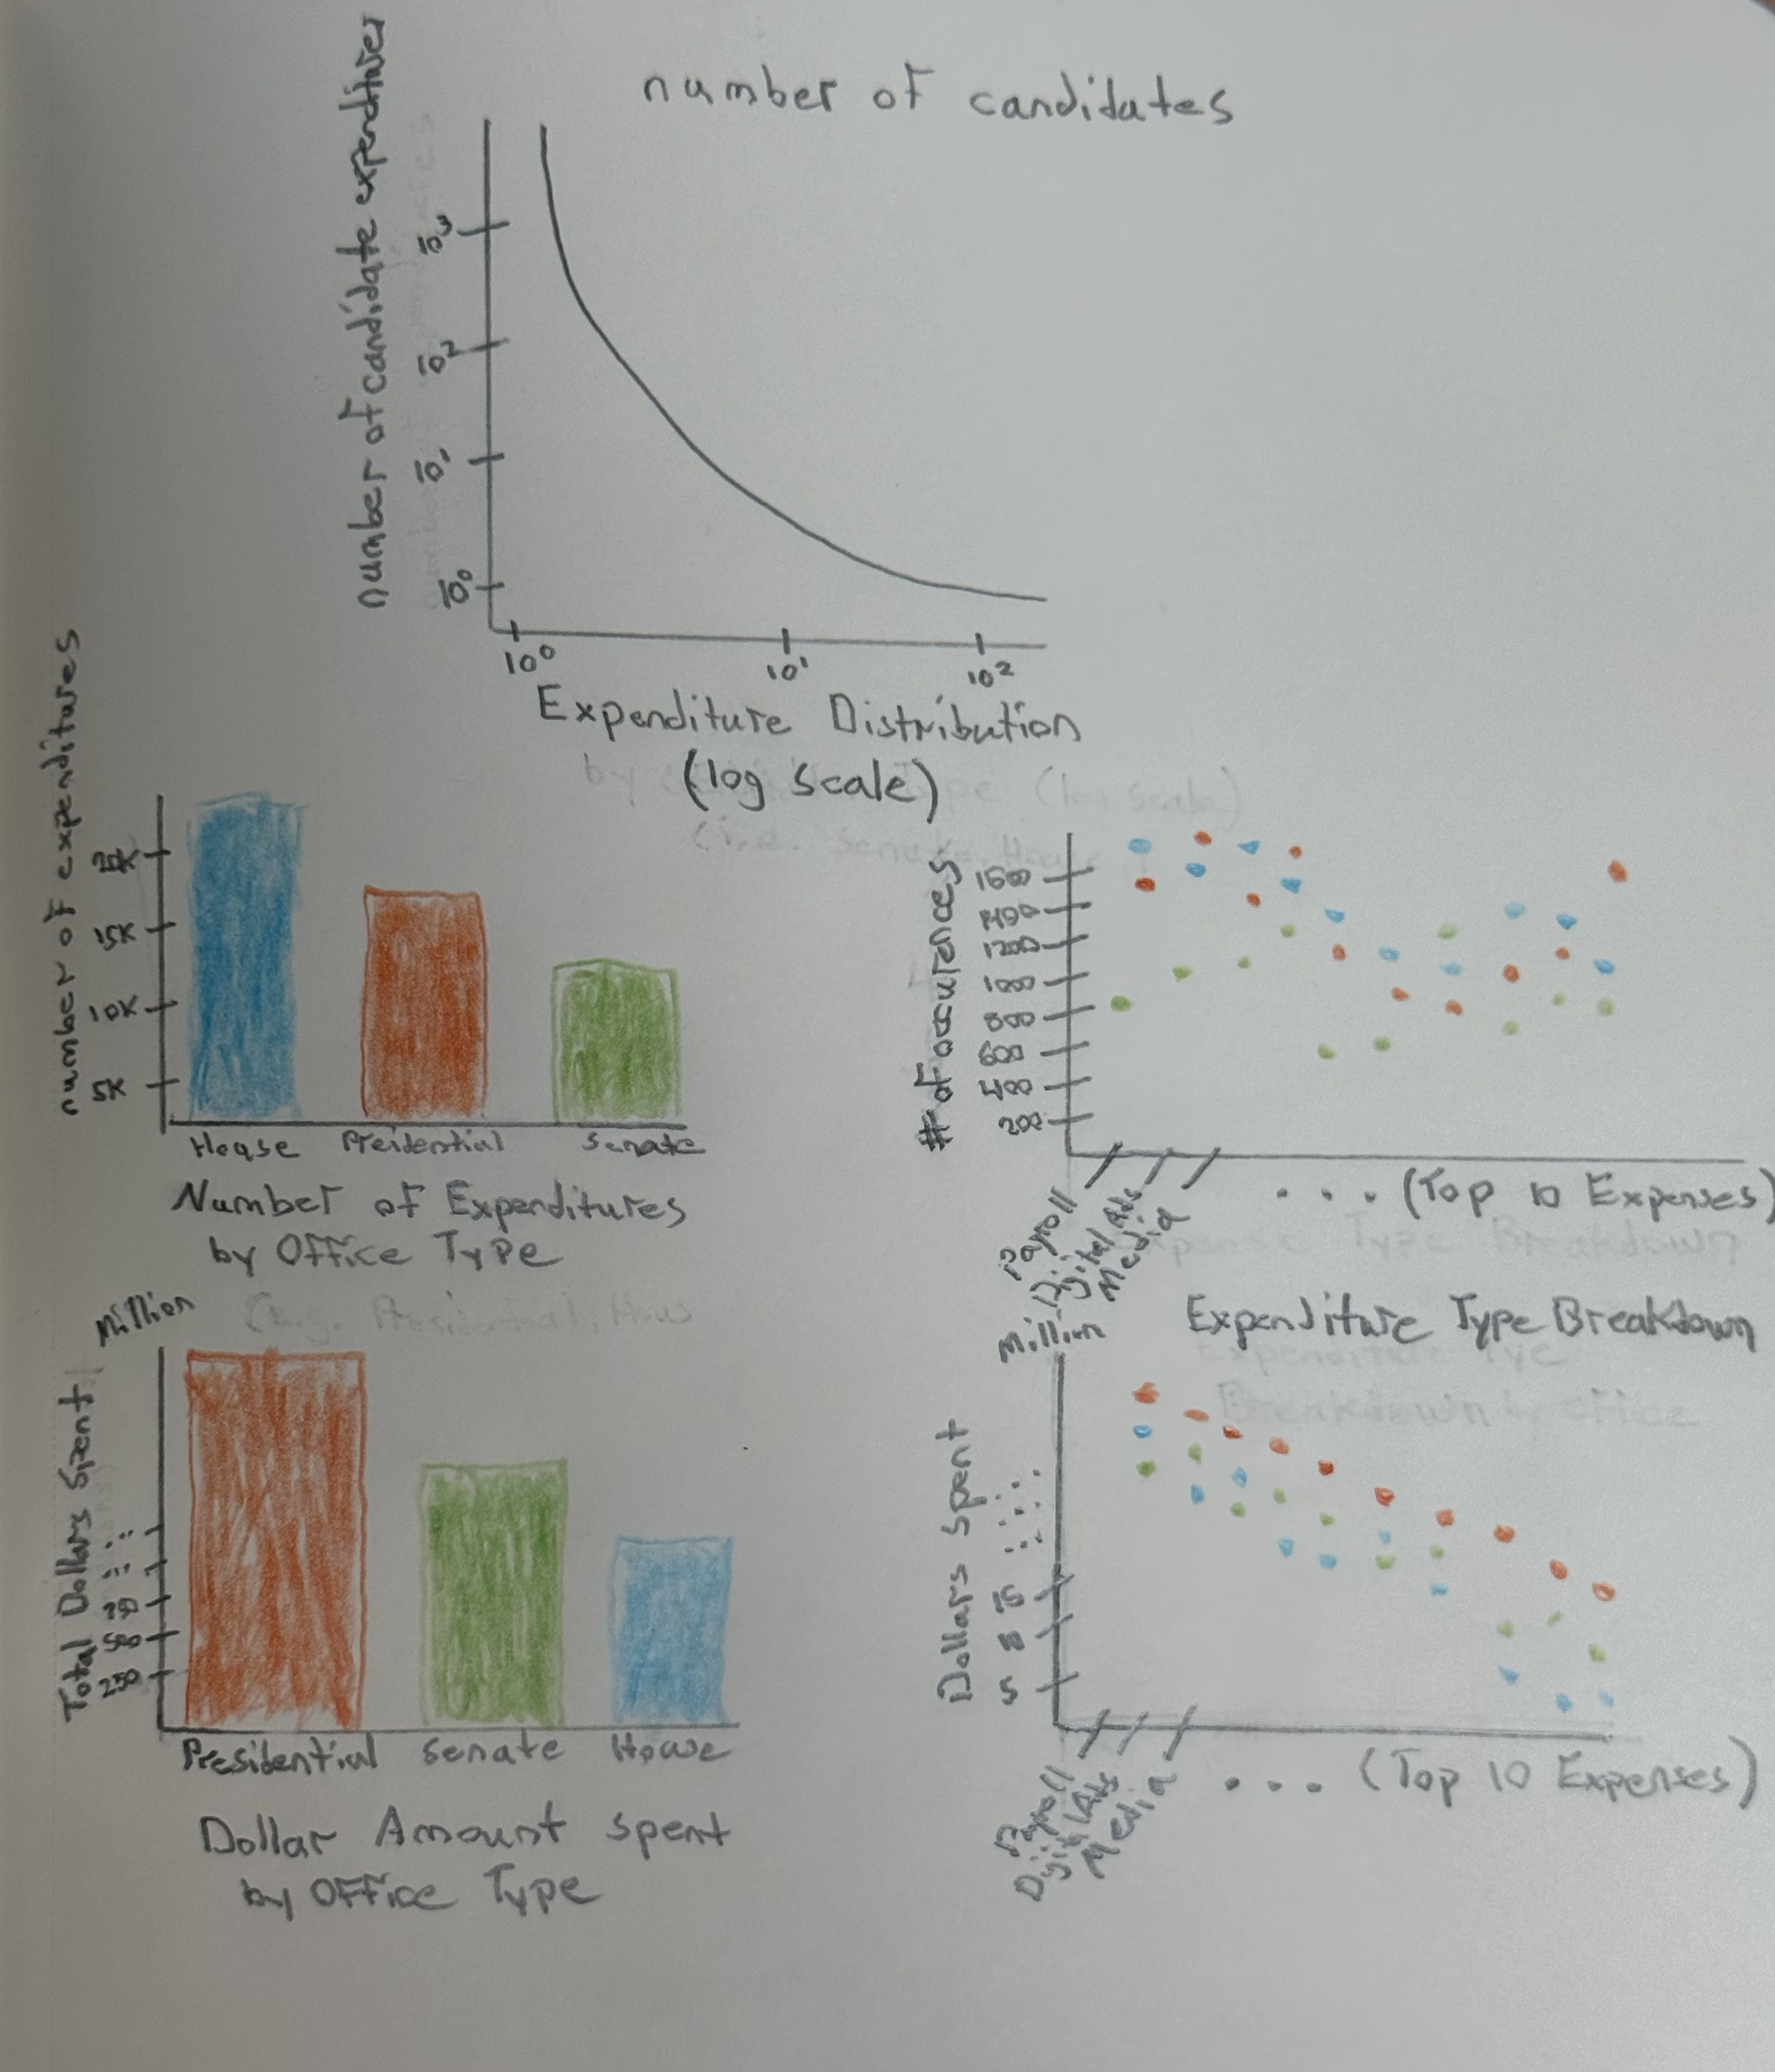
\includegraphics[width=0.8\linewidth]{DS_HW3_hand_drawn.jpeg}
    \caption{A Visually Consistent Plot}
    \label{fig:myfigure}
\end{figure}

In the image above, I start with a cleaner-looking power law distribution by flipping the axis and smoothing out the tail. In the plots below, presented in a top-to-bottom, left-to-right fashion, I begin to unpack and answer the questions that emerged from the provided feedback. First, more context is provided on the expenditure distribution by breaking it down by House, Senate, and Presidential race types. Then the viewer can better understand the actual nature of expenditures through frequency analysis. Finally, we translate expenditures into dollars, following the same narrative structure. Each plot provides a key piece of information that helps tell a bigger story.

What the viewer must keep in mind while interpreting this data is that there were primarily 2 presidential candidates in this dataset, compared to hundreds of House and Senate candidates. As one navigates these visualizations with this context in mind, the true magnitude of presidential elections in this country becomes apparent—not only in terms of money, but in human effort and organizational complexity as well.

\subsection*{Part 2: Translate hand drawn image to plot}

Below there are 3 iterations. The first plot shows a lack of success in the scatter plots due to a lack of consistency across expenditure types.

\begin{figure}[h!]
    \centering
    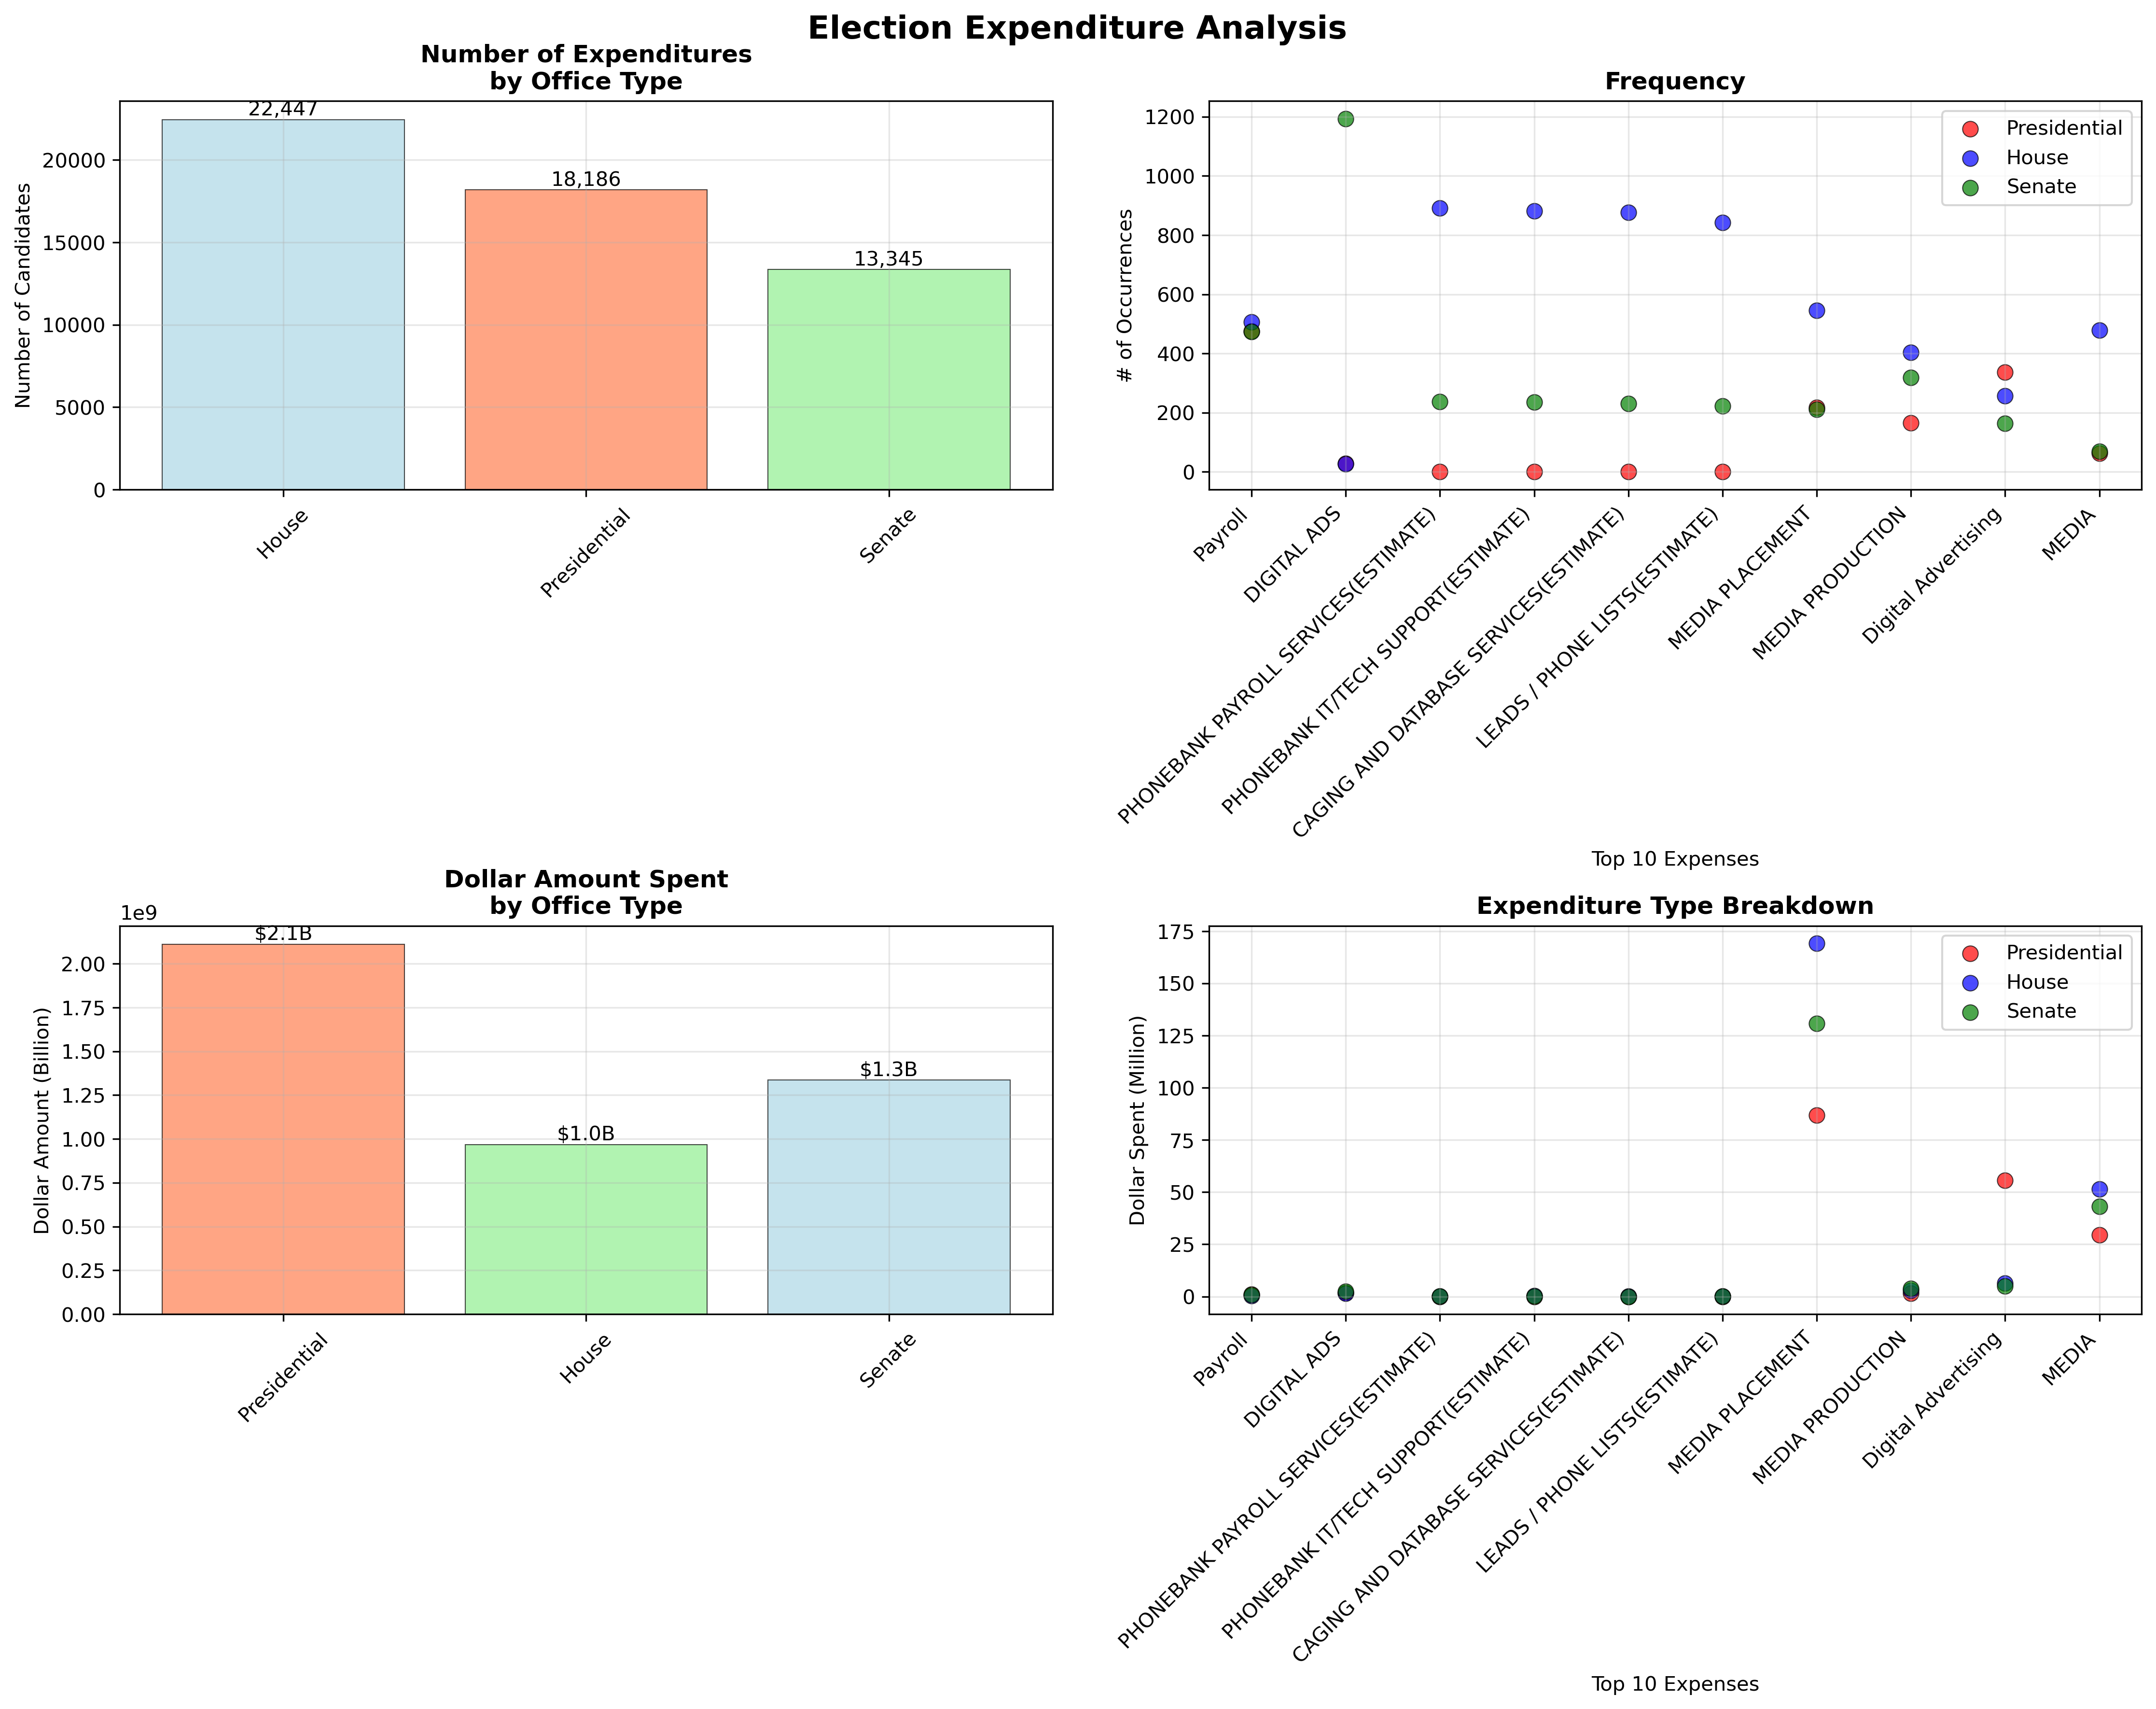
\includegraphics[width=0.8\linewidth]{election_expenditure_analysis_iteration_1.png}
    \caption{Iteration 1}
    \label{fig:myfigure}
\end{figure}

To address the lack of consistency I decided to create horizontal bar plots that displayed spending for presidential and non-presidential (house and senate) office types. The idea being that the flow would go as follows:

expenditure breakdown count by office type -> translate expenditure counts to money spent -> breakdown the way the money is spent by office types

\begin{figure}[h!]
    \centering
    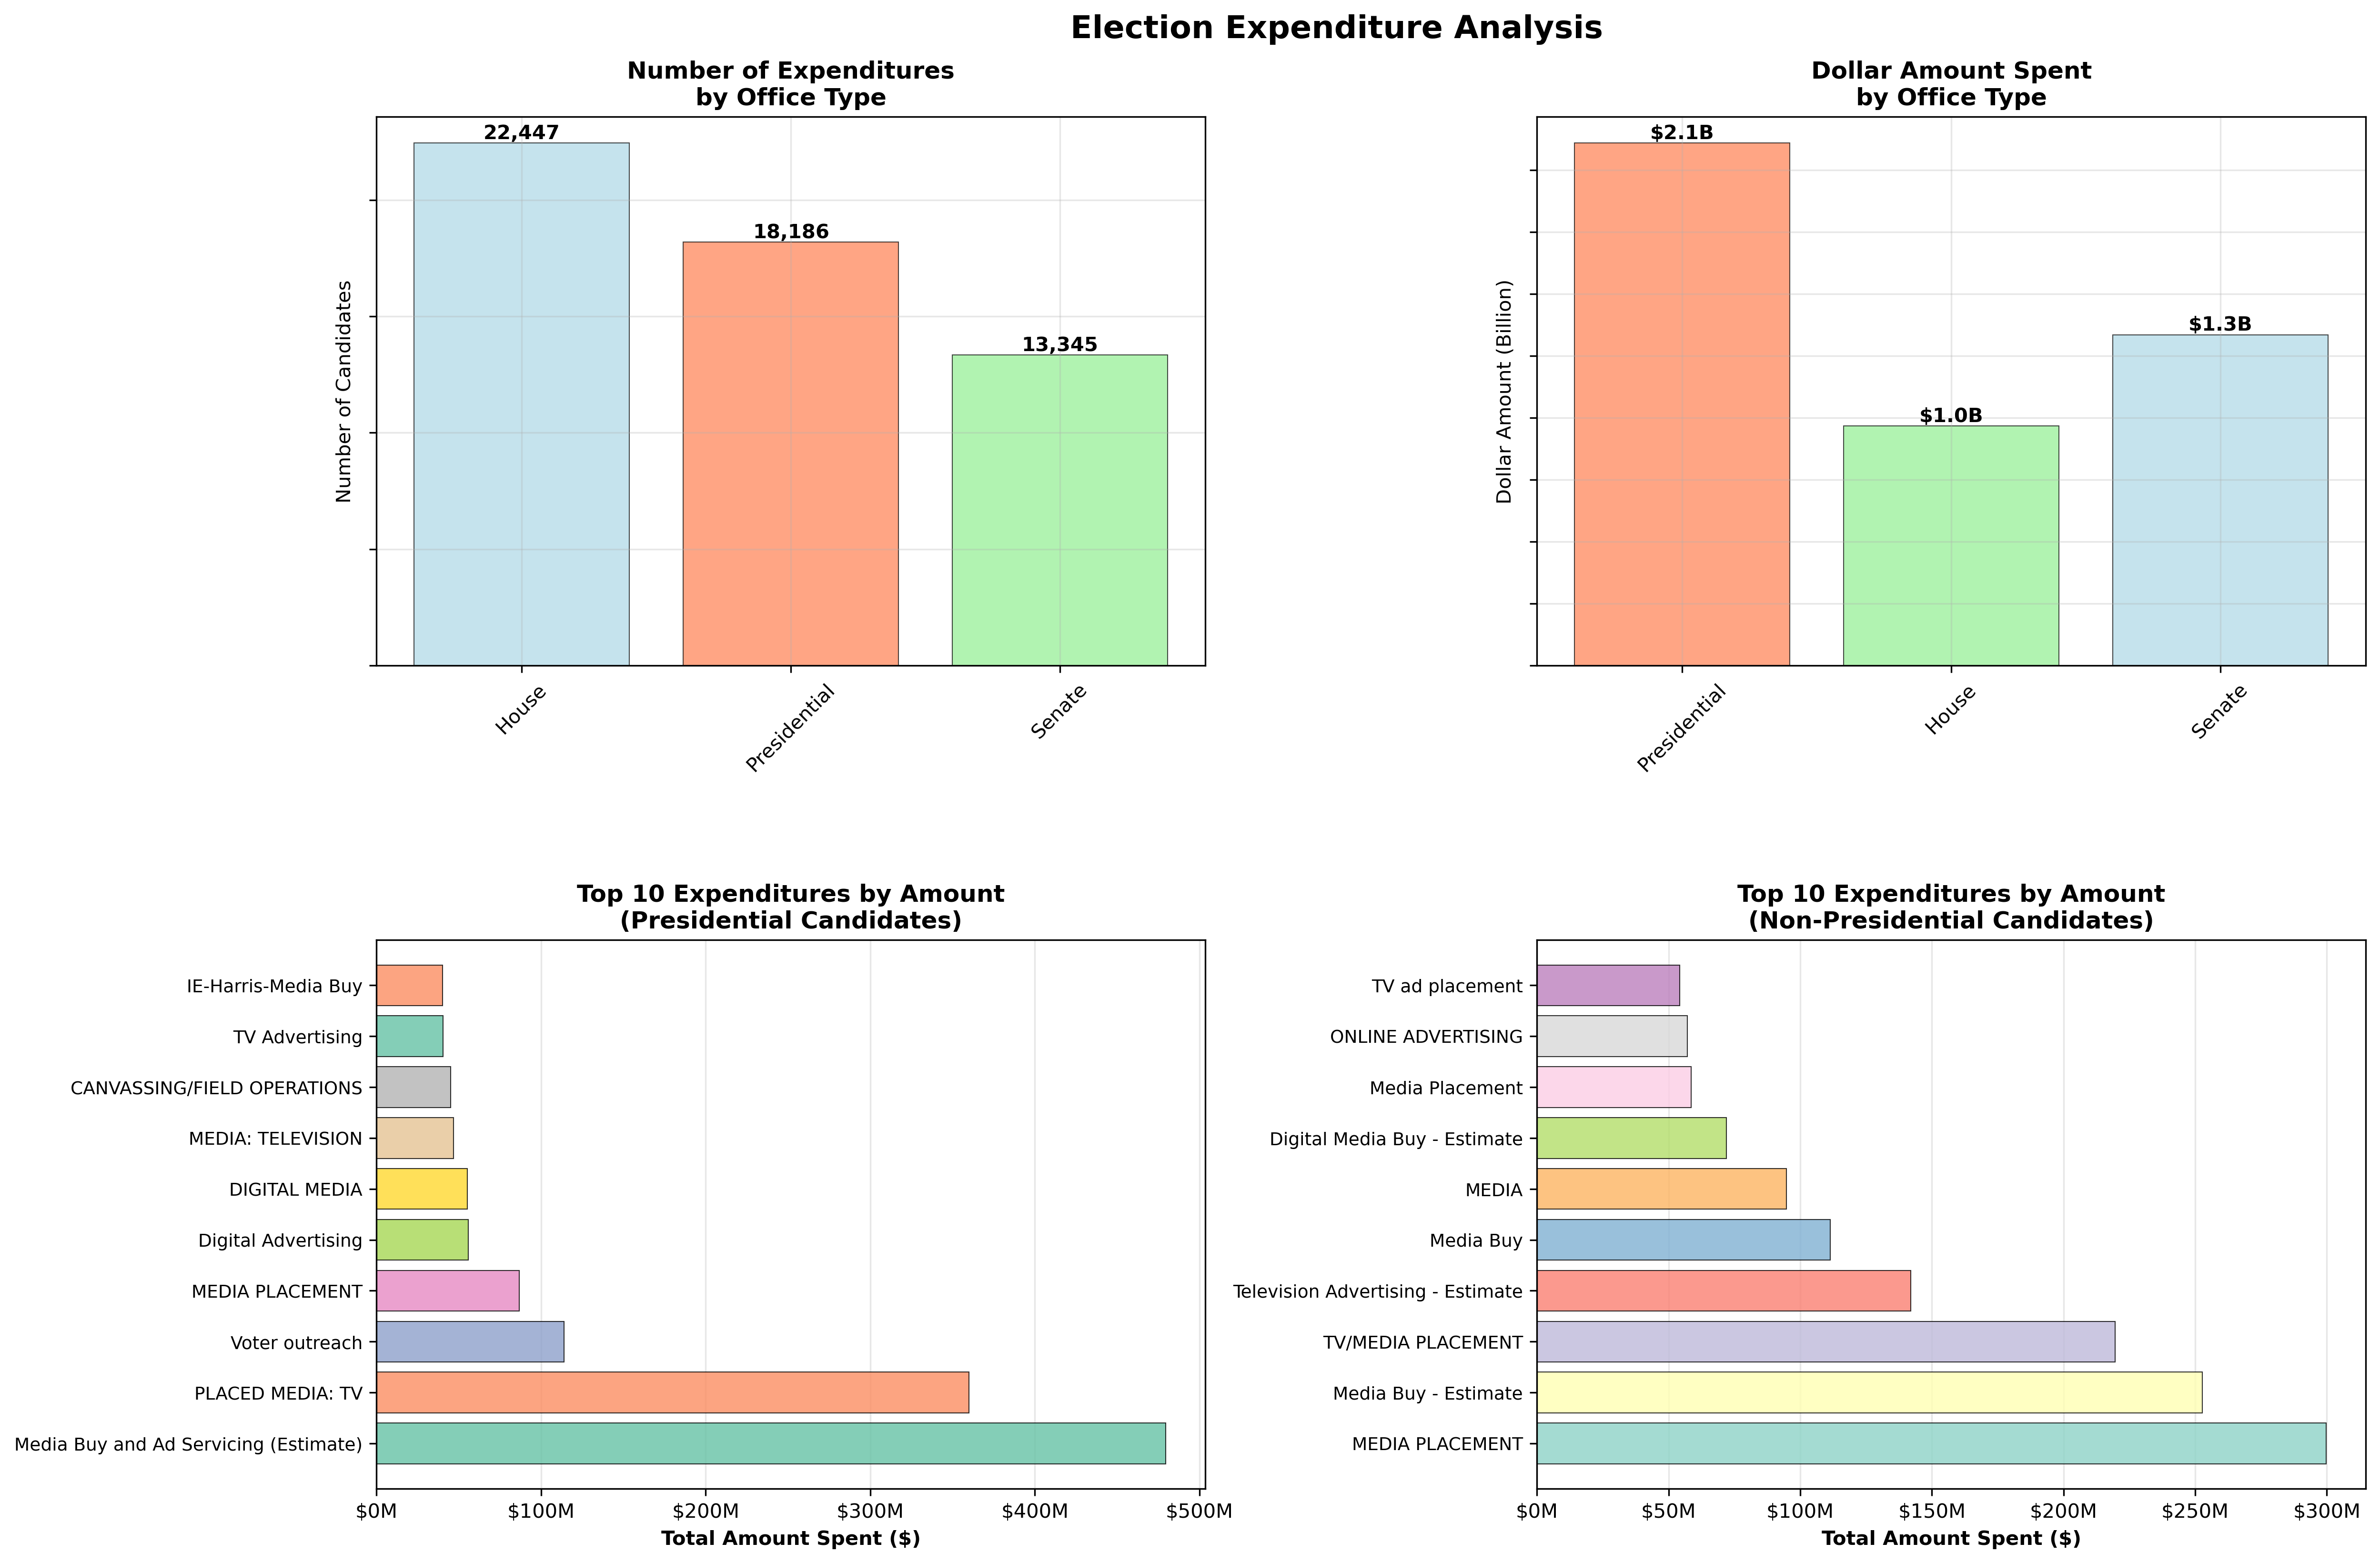
\includegraphics[width=0.8\linewidth]{election_expenditure_analysis_iteration_2.png}
    \caption{Itreation 2}
    \label{fig:myfigure}
\end{figure}

However, I still found this approach a bit confusing, and I felt it didn't address the questions I set out to answer with these plots. Also, I felt that I totally failed to achieve a visually consistent language. What follows is something much nicer!

\begin{figure}[h!]
    \centering
    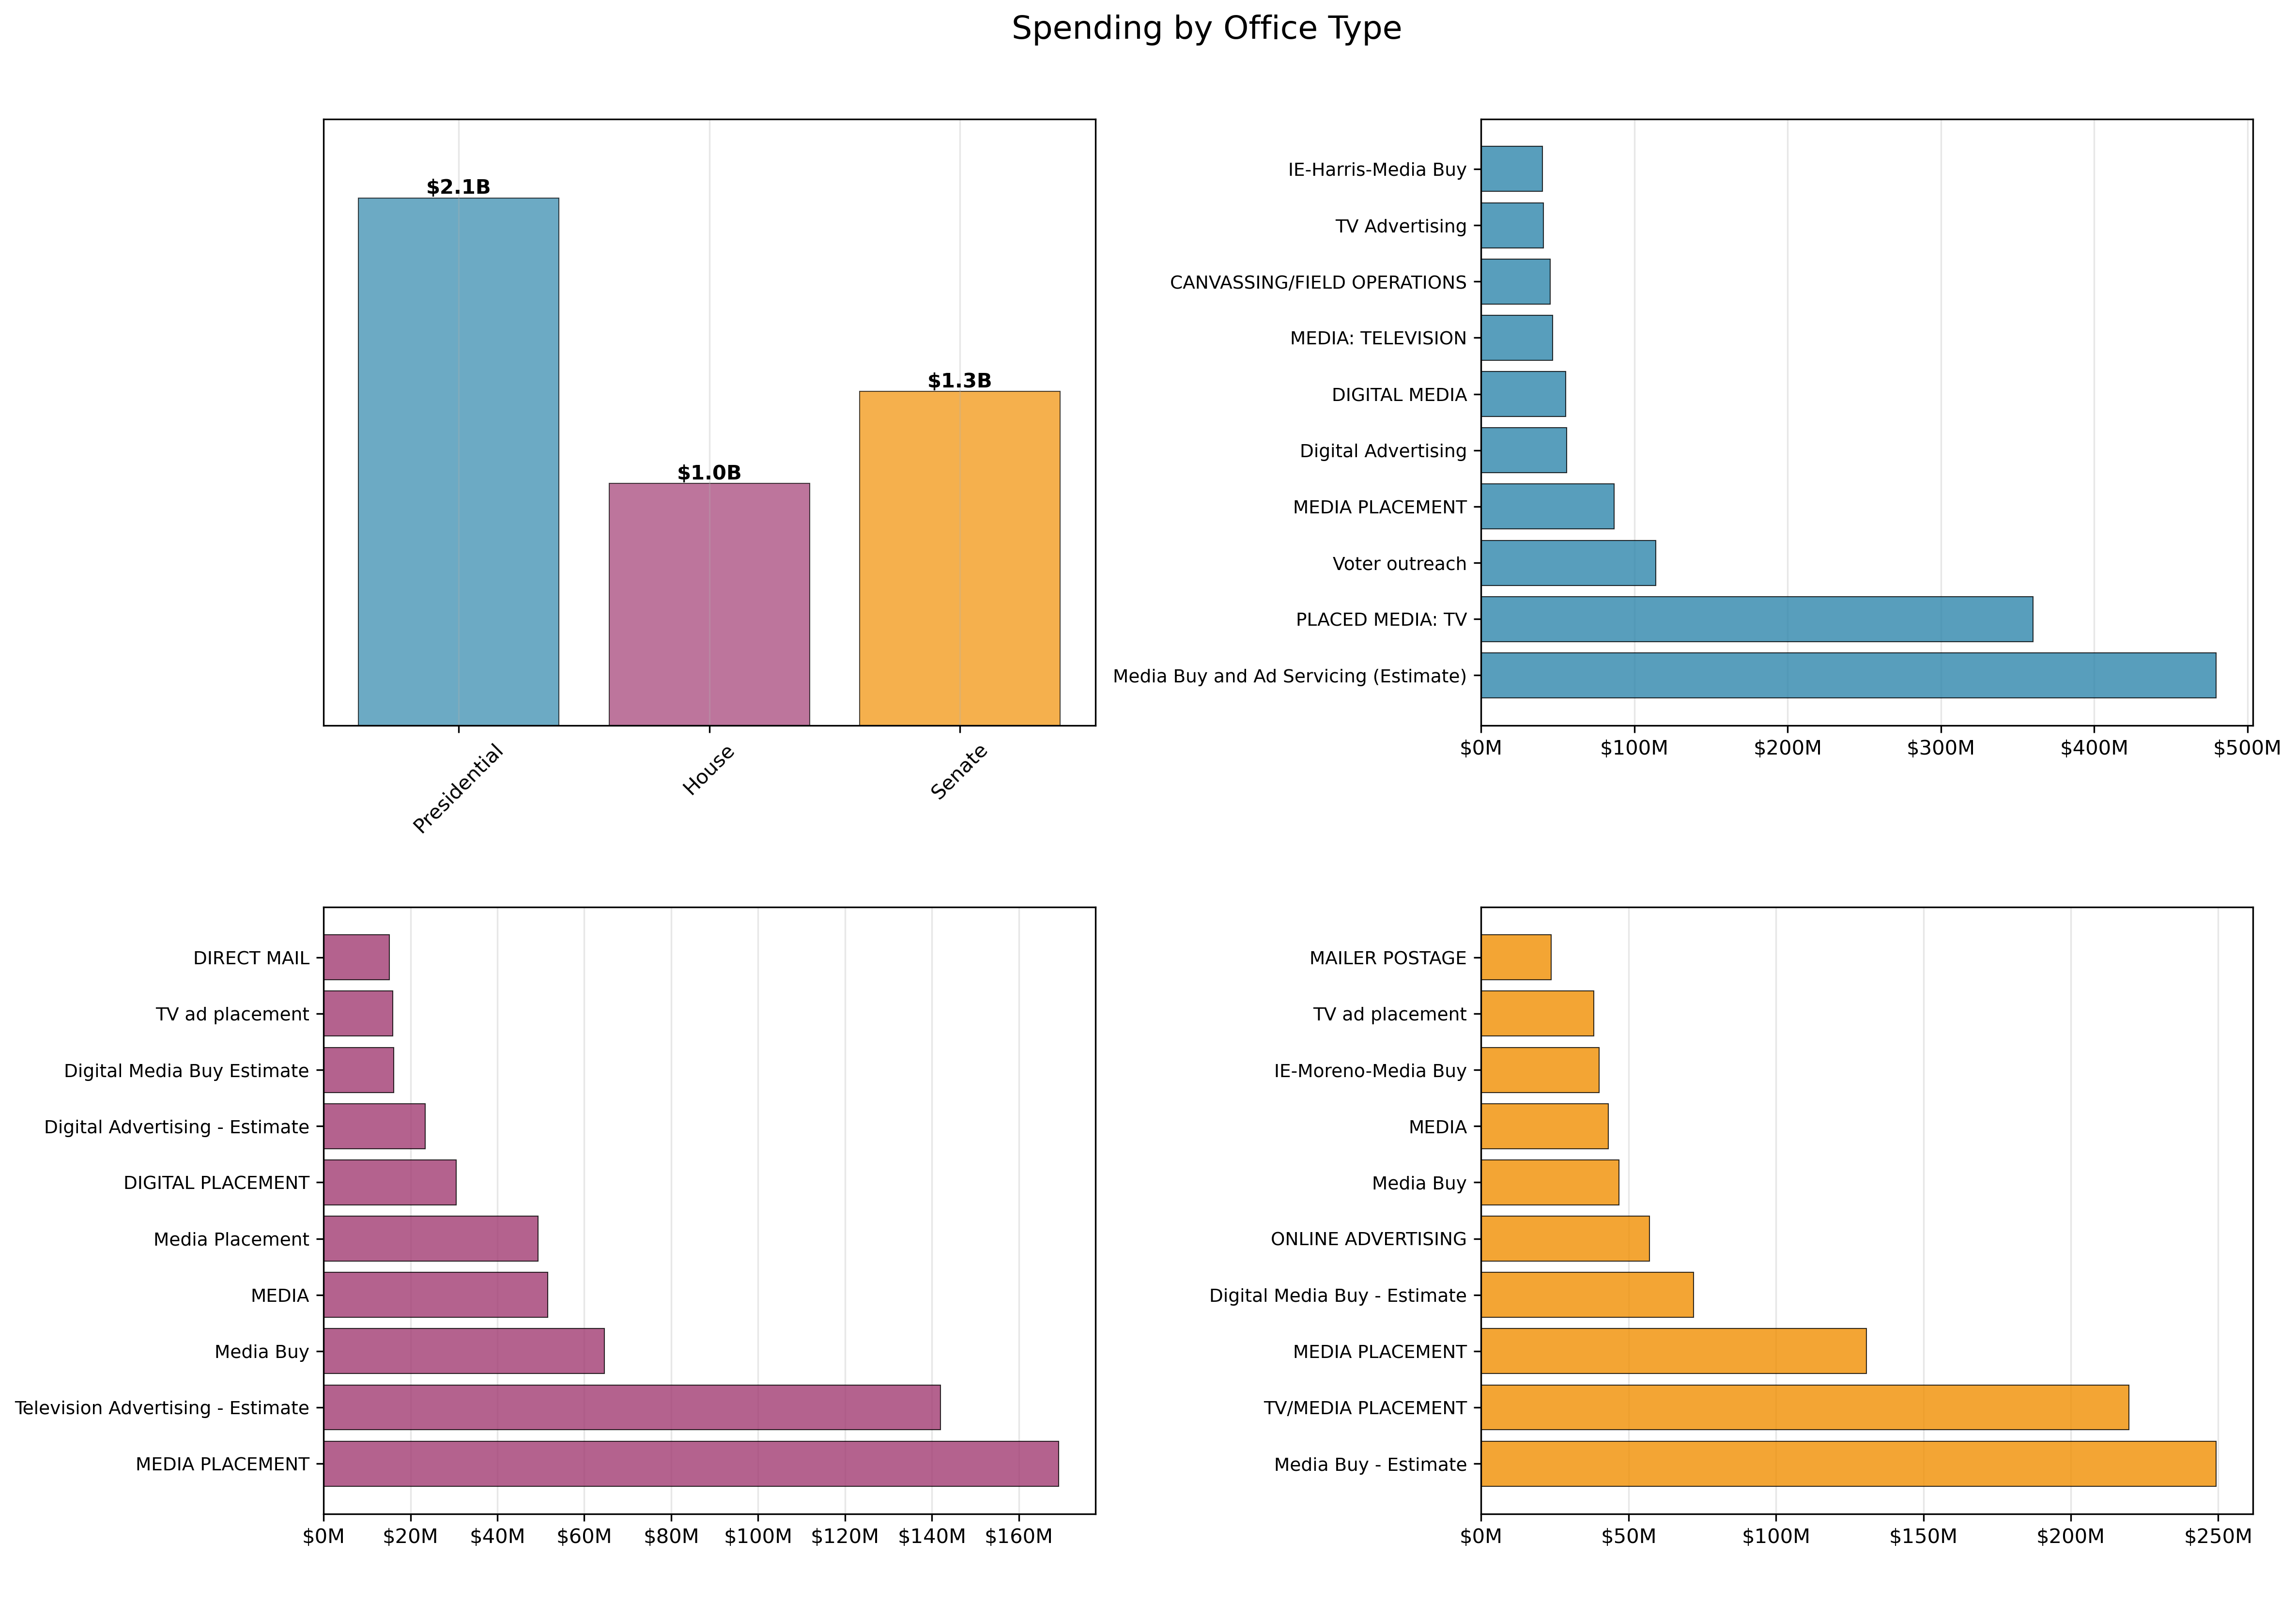
\includegraphics[width=0.8\linewidth]{election_expenditure_analysis_iteration_3.png}
    \caption{Iteration 3}
    \label{fig:myfigure}
\end{figure}

Above we see much cleaner panel! It focuses entirely on spending and doesn't confuse the viewer by making the transition from count expenditures to how those translate into dollars. Also I removed titles as I felt the plots were self-explanatory. One criticism I have of this panel is that I still haven't gotten a sense of how to manipulate fonts. I would love to be able to select a font that better matches the overall aesthetic.

\section*{Question 2: Causal Statements}

\subsection*{Statement 1}

\textbf{Causal Statement:} "There are certain groups of people that don't take vaccines and don't take any pills and have no autism." - Donald Trump

\begin{center}
\begin{tikzcd}
	{\text{Certain Groups}} & {\text{No Vaccines}} \\
	{\text{No Pills}} & {\text{No Autism}}
	\arrow[dotted, from=1-1, to=1-2]
	\arrow[dotted, from=1-1, to=2-1]
	\arrow[from=1-2, to=2-2]
	\arrow[from=2-1, to=2-2]
\end{tikzcd}
\end{center}

\subsubsection*{Analysis Questions:}

\textbf{Counterfactual:}

The implicit counterfactual here is that if certain groups (e.g. "The Amish") vaccinated and took pills, they would have autism in their population.

\vspace{0.5in}
\textbf{Ideal Experiment:}

An ideal experiment here would be to research communities where access to Tylenol and vaccines is limited by socioeconomic circumstances rather than a belief system. This kind of experiment would be generational and track groups that engaged with Tylenol, vaccines, both as well as a control group.

\vspace{0.5in}
\textbf{Potential Confounds:}
\begin{itemize}
    \item Socioeconomic status: Wealthier families may be more likely to both avoid vaccines AND have better access to early autism diagnosis/services
    \item Education/beliefs: Parents who avoid vaccines may also avoid seeking autism diagnoses due to stigma or distrust of medical establishment
\end{itemize}
\vspace{0.5in}

\subsection*{Statement 2}

\textbf{Causal Statement:} Democrats are about to shutdown the government because they demand we fund healthcare for illegal aliens." - JD Vance

\begin{center}
\[\begin{tikzcd}
	& {\text{Democrats}} \\
	& {\text{fund healthcare}} \\
	{\text{non-citizens}} && {\text{citizens}} \\
	& {\text{government shutdown}} && {\text{government does not shutdown}} \\
	&& {\text{loss of essential services for all}}
	\arrow[from=1-2, to=2-2]
	\arrow[from=2-2, to=3-1]
	\arrow[from=2-2, to=3-3]
	\arrow[from=3-1, to=4-2]
	\arrow[from=3-3, to=4-4]
	\arrow[from=4-2, to=5-3]
\end{tikzcd}\]
\end{center}

\subsubsection{Analysis Questions:}

\textbf{Counterfactual:}

The reverse implication of this statement would be that Democrats do not fund healthcare for non-citizens and the government stays open.

\vspace{0.5in}

\textbf{Potential Confounds:}
\begin{itemize}
    \item Budget negotiations complexity: A shutdown might ultimately occur due to a failure to negotiate a multitude of complex issues. Publ 
    \item Public opinion: This may be an effort to pressure Democrats to cave by controlling the narrative.
    \item Distraction: This could be an effort to distract from actual healthcare funding disputes (Medicare, Medicaid, ACA tax credits).
\end{itemize}

\vspace{0.5in}

\subsection*{Statement 3}

\textbf{Causal Statement:} "Marvel is better than DC because they have less stereotypical superhero ideas like The Thing versus Superman. The Thing's powers can impede him. They stop him from living a normal life because of his rock-like skin and monstrous appearance, but Superman has all the benefits of being a superhero - speed, superhuman strength, but none of the downsides."

\begin{center}
\begin{tikzcd}
	{\text{Superheros}} & {\text{Flaws}} & {\text{Character Depth}} & {\text{Story Quality}} \\
	{\text{The Thing - Marvel}} & {\text{rock-like skin and monstrous appearance}} & {\text{Complex character}} & {\text{Better}} \\
	{\text{Superman - DC}} & {\text{No apparent flaws}} & {\text{Simpler character}} & {\text{Worse}}
	\arrow[from=1-1, to=1-2]
	\arrow[from=1-1, to=2-1]
	\arrow[from=1-2, to=1-3]
	\arrow[from=1-3, to=1-4]
	\arrow[from=2-1, to=2-2]
	\arrow[from=2-2, to=2-3]
	\arrow[from=2-3, to=2-4]
	\arrow[from=3-1, to=3-2]
	\arrow[from=3-2, to=3-3]
	\arrow[from=3-3, to=3-4]
\end{tikzcd}
\end{center}

\subsubsection*{Analysis Questions:}

\textbf{Counterfactual:} 

 If DC characters had superpowers balanced with flaws (like The Thing), their characters would have more depth, and their stories would be better.

\vspace{0.5in}

\textbf{Ideal Experiment:}

Create an extensive and agreed upon rubric for evaluating the complexity and depth of superheros and apply it to Marvel and DC.

\vspace{0.5in}

\textbf{Potential Confounds:}
\begin{itemize}
    \item Fan community expectations: Fans of superheros might have developed certain norms and expectations of characters over time.
    \item Artistic talent: Individual writer/artist quality may matter more than publisher philosophy - Jerry Siegel/Joe Shuster vs. Stan lee/Jack Kirby
    \item Cherry-picking examples: Selecting specific character pairs (Thing vs Superman) rather than representative samples.
    \item Publication era effects: Characters created in different time periods may reflect different norms, conventions, expectations, and behaviors.
\end{itemize}
\vspace{0.5in}
\end{document}


\textbf{Counterfactual:} 

 If DC characters had superpowers balanced with flaws (like The Thing), their characters would have more depth, and their stories would be better.

\vspace{0.5in}

\textbf{Ideal Experiment:}

Create an extensive and agreed upon rubric for evaluating the complexity and depth of superheros and apply it to Marvel and DC.

\vspace{0.5in}

\textbf{Potential Confounds:}
\begin{itemize}
    \item Fan community expectations: Fans of superheros might have developed certain norms and expectations of characters over time.
    \item Artistic talent: Individual writer/artist quality may matter more than publisher philosophy - Jerry Siegel/Joe Shuster vs. Stan lee/Jack Kirby
    \item Cherry-picking examples: Selecting specific character pairs (Thing vs Superman) rather than representative samples.
    \item Publication era effects: Characters created in different time periods may reflect different norms, conventions, expectations, and behaviors.
\end{itemize}
\vspace{0.5in}
\end{document}
